\section{Qualitative Analysis - Quasi-Free Scattering $^{12}$C(p,2p)$^{11}$B}
Until the S444 experiment in 2020 CALIFA consisted out of a prototype frame filled with up to 64 CsI(Tl) crystals. The geometric coverage was therefore limited. For the S444 experiment CALIFA got its final frame and was fully filled in the forward barrel and 35\%filled in the iPhos region, CEPA was not installed yet. With these improvements it was possible to commission QFS-experiments with CALIFA at R$^3$B. In the follow up experiment S467, also in 2020, the first experimental run to study single-particle structures of neutron-rich Ca isotopes via QFS reactions was carried out.\newline
Even though great improvements in the detector development  were achieved the correction factors to correct for geometric acceptance would be much too high ( $\approx$ 10) for precise cross section measurements for QFS-reactions since the correction factors would in turn rely on a a simplified reaction model. A precise analysis of the acceptance correction factor and the development of a more sophisticated and data driven reaction model is out of the scope of this work. Therefore this analysis focusses on the methods of QFS-reaction identification and the extraction of the key informations dicussed in section \ref{sec:qfs_theo}. TODO: add more stuff here...\newline
\subsection{Setup-Calibration}
For setup description refer to section \ref{sec:analysis_cross_sec}. For all detectors except the SOFIA (Study On FIssion with Aladin) Time of Flight Wall the calibration parameters investigated by the respective detector-expert group were adopted. Herefore we will subsequently only describe the Time of Flight Wall calibration in this subsection.
\subsubsection{Flight-Path Reconstruction}\label{subsec:flightpath_reco}
The procedure to calibrate the Time of Flight (ToF) Wall involves beforehand a precise flight-path reconstruction of the projectile from the entrance of Cave C downstream to the ToF Wall. Since only one tracking detector downstream to GLAD was in operation for the S444 experiment no angle of the deflected fragment/beam $\theta_{out}$ could be directly extracted. Herefore an advanced tracking algorithm was developed, motivated from ref. \cite{bertini2013study} (section 3.4). 
\begin{itemize}
\item The first step is to measure the scattering angle after target, $\theta_{in}$, and draw an extended line from the target position through the effective magnetic field of GLAD.  
\item Draw a trajectory line from the hit position in MWPC3 to the intersection point C (see figure \ref{fig:sub1_reco_path}) of the "kick-plane-line" and the reconstructed and extended track line upstream to GLAD.
\item Now sweep along the reconstructed track line upstream to GLAD. For each step a value for $\theta_{out}$ and $d1-d2$ is gathered, see figure \ref{fig:sub2_reco_path}.
\item As in figure \ref{fig:sub2_reco_path} shown, fit the data-points from previous step with a linear fit function and find the corresponding $\theta_{out}$ value where the fit line intersects with the abscissa. This corresponds to the case where $d1 = d2$. This is the approximated "kickpoint" in GLAD. 
\item Previous steps need to be executed for all events accordingly.
\end{itemize}
\begin{figure}[ht]
    \centering
    % First subfigure
    \begin{subfigure}[b]{0.70\textwidth}
		\centering
        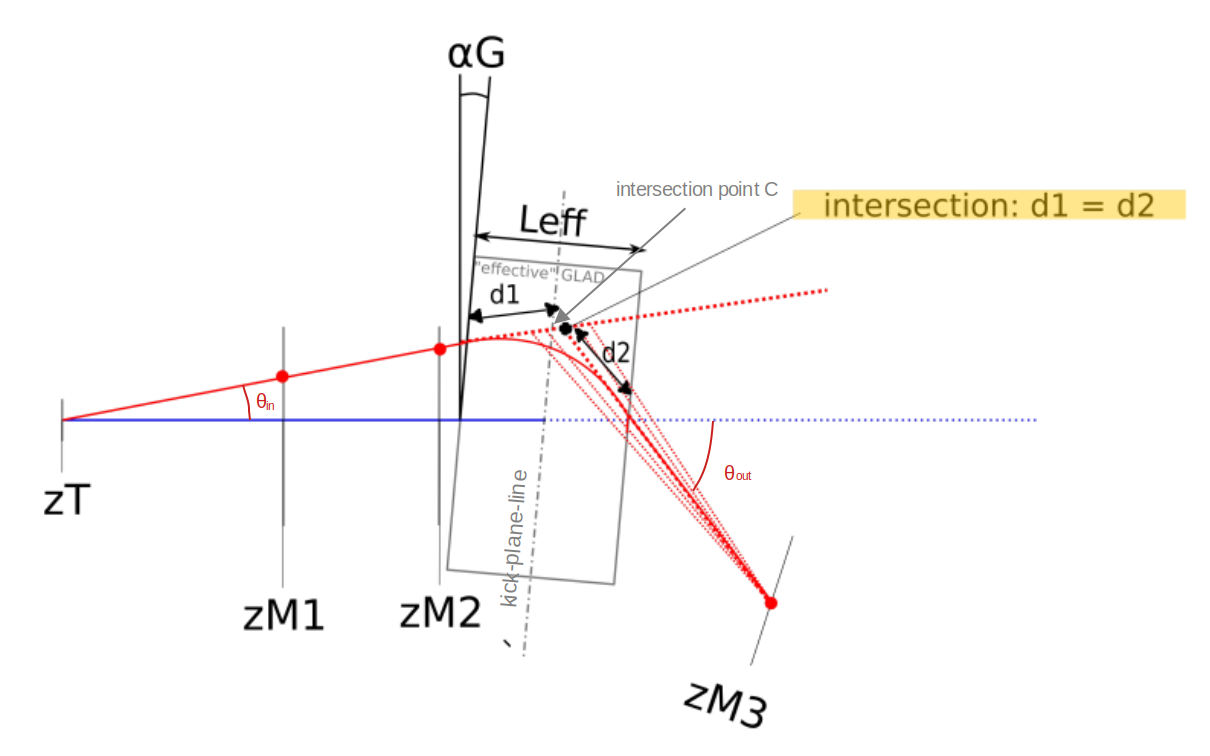
\includegraphics[width=\textwidth]{Figures/kick_point_algorithm.png}
        \caption{Flightpath reconstruction with "Leff" being the effective active width of the magnetic field of GLAD}
        \label{fig:sub1_reco_path}
    \end{subfigure}
    %\hfill % Optional: adds horizontal space between the figures
    % Second subfigure
    \begin{subfigure}[b]{0.25\textwidth}
		\centering
        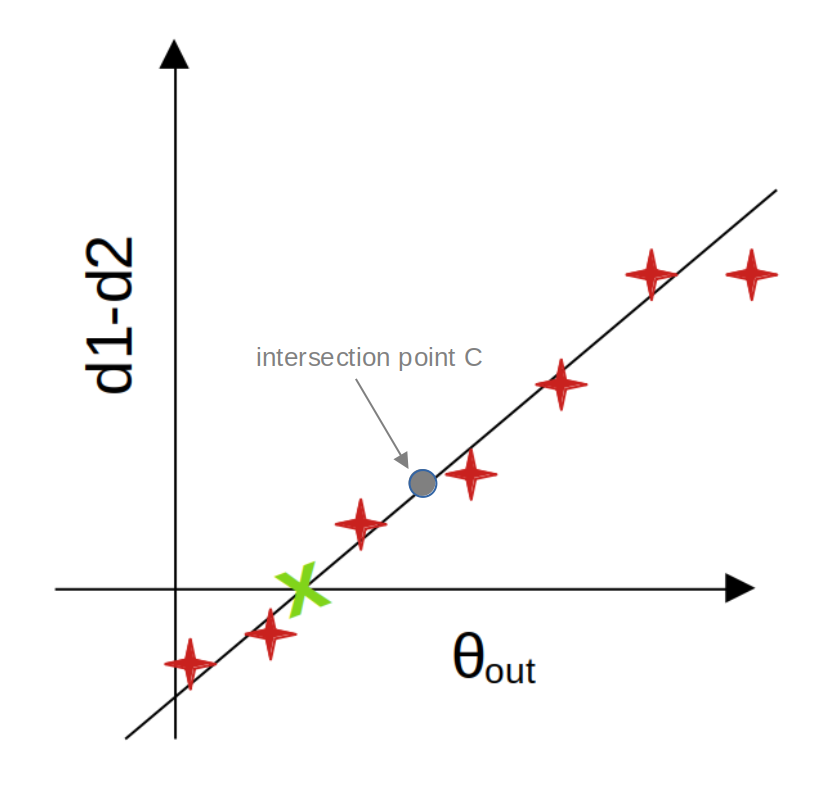
\includegraphics[width=\textwidth]{Figures/intersection_algorithm.png}
        \caption{$\theta_{out}$ approximation. For detailed information see text.}
        \label{fig:sub2_reco_path}
    \end{subfigure}

    \caption{Flightpath tracking and reconstruction of the fragment/beam after the target.}
    \label{fig:reco_path}
\end{figure}

Now that the scattering angle after the target $\theta_{in}$ and the angle after GLAD, $\theta_{out}$ is known and the position outside the magnetic field of GLAD are fixed, with $(z_1,x_1)$  the entrance point on the GLAD field and $(z_2,x_2)$ the exit point, the bending radius $r$ from the magnetic deflection can be determined:
\begin{equation}\label{eq:rho_glad}
r = \frac{L_{eff}}{2\,\cdot sin\left(\frac{\theta_{in}+\theta_{out}}{2}\right)\,\cdot cos\delta}
\end{equation}
where $L_{eff}$ is the effective active with of the magnetic field of GLAD, which correspons $L_{eff} \approx 2.06\,m$. This value could also be verified by extracting $L_{eff}$ from the formula for the magnetic rigidity $ B\cdot r = \gamma\beta \, m /q$ for empty target runs with known values of the B-field\footnote{For detector calibration, primarly for the ToFWall, we had several "empty sweep runs", with empty target and different B-field strenght settings. Those runs were optimal to validate $L_{eff}$.}.\newline
The angle $\delta$ in equation \ref{eq:rho_glad} is given by the trajectory line going through $(z_1,x_1)$/$(z_2,x_2)$ and the line parallel to the GLAD magnet width $L_{eff}$.\newline
A detailed derivation of equation \ref{eq:rho_glad} can be found in appendix \ref{app:flightpath}.
The arc trajectory $l_{GLAD}$ of the fragment within GLAD can be reconstructed using the bending radius $r$ and the entry and exit points $(z_1,x_1)$/$(z_2,x_2)$:
\begin{equation}\label{eq:arc}
l_{GLAD} = r \cdot \omega\qquad \text{with}\qquad \omega = 2\cdot asin(t_{1/2}{(2\cdot r)})
\end{equation}
where $\omega$ is the central angle and  $t_{1/2}$ is the cord length between $(z_1,x_1)$ and $(z_2,x_2)$.\newline
At this stage the full pathlength $L$ form the Start detector to the ToFW is fixed:
\begin{description}
\item \textbf{From Start to the target $l_{ST}$:} For this path section a straight flightpath parallel to the z-coordinate is assumed. The pathlength is taken from the position measurements of the Start detector and the target accordingly ($=118.3\,cm$). 
\item \textbf{Target to GLAD entrance point $(z_1,x_1)$, $l_{in}$:}For the  exact position assignment of $(z_1,x_1)$ both MWPC1 and MWPC2 position measurements have been calibrated with empty target runs by including an offset valuein order to center the x-position in both detectors around zero. From the position measurement of the central position of GLAD, its tilting angle $\alpha$ and $L_{eff}$ the intersection point of the fragment trajectory before GLAD and the "effective GLAD magnetic field rectangle", $(z_1,x_1)$, can be determined and with it the according flightpath section $l_{in}$.
\item \textbf{Arc trajectory within GLAD, ${l_{GLAD}}$:}This flightpath passage is determined by reconstructing $(z_1,x_1)$ and $(z_2,x_2)$, as it has been described in detail in the previous section. Hence the magnetic bending radius can be determined, see equation \ref{eq:rho_glad}, and finally the arc trajectory ${l_{GLAD}}$ as in equation \ref{eq:arc}.
\item \textbf{GLAD exit point $(z_2,x_2)$ to ToFW, $l_{out}$:}The hit position $(z_{MWPC3},x_{MWPC3})$ in MWPC3 is given by the reconstructed hit position in this detector and the position measurement of the detector itself. The exit point $(z_2,x_2)$ was reconstructed in the previous steps. Hence the trajectory line from $(z_2,x_2)$ to $(z_{MWPC3},x_{MWPC3})$ is fixed and is expanded to the intersection with the ToFW plane for the concluding $l_{out}$ measurement.  
\end{description}
The resulting flightpath $L$ recombines from:
\begin{align*}
L &= l_{ST}+l_{in}+l_{GLAD} + l_{out} 
\end{align*}
In the flightpath reconstruction the deflections in the y-dimension were omitted as the angular straggling in the target is small (TODO: give sigma value) and since the deflection of the fragment within GLAD is independent from its  y-position this contribution can be disregarded.


\subsubsection{Time of Flight Calibration}
For the time of flight measurement in the S444 setup the time is recorded and digitized by the VFTX,  VME-FPGA Time-to-Digital Converter (TDC) Modules based on tapped delay line (TDL) TDCs\cite{bayer2009development}. These modules provide for each detected signal a coarse time, is determined by counting cycles of a 200 MHz readout clock, resulting in a 5 ns binning resolution, and a fine time, which is obtained using an FPGA-based Time-to-Digital Converter (TDC), which employs a tapped delay line (TDL). In this approach, the signal propagates through a series of delayed logic modules within the FPGA until the subsequent clock cycle terminates the sampling process. The number of delay elements traversed by the signal is used to compute the time difference between the signal onset and the end of the clock cycle. The translation of the resulting fine time, with reasonable assumption of an uniform distribution, is achieved via a calibrated linear function. This procedure assigns to each preamplifier signal in the start detector (left/right) and the ToF Wall (up/down) a calibrated raw time \textit{raw\_t}:
\begin{align*}
raw\_t &= coarse\_time\_clocks  \cdot 5ns + offset[fine\_time]
\end{align*}
Finally, the raw time of flight is reconstructed by combinding all four time measurements:
\begin{gather}
RawTof = 0.5*(raw\_t_{i,down}+raw\_t_{i,up}) - 0.5*(raw\_t_{start,right}+raw\_t_{start,left})
\end{gather}
where \textit{i} $(\in 0...27)$ refers to the scintillator number of the ToF Wall. Since the mentioned time measurements are standalone and not synchronized the \textit{RawToF} has to be corrected by an offset which has to be determined again for each scintillator bar \textit{i} of the ToF Wall:
\begin{align*}
\Delta_{ToF}[i] &= \overline{L[i]}/v_{beam} - \overline{RawTof[i]}
\end{align*} 
where $\overline{L[i]}$ is the mean reconstructed path length for all events in empty target runs which hit scintillator bar \textit{i} of the ToF Wall. The beam velocity $v_{beam}$ is directly taken from the given beam settings, e.g. 400 AMeV beam, emtpy target corresponds to $v_{beam} = 214,2mm/ns$. The mean raw ToF $\overline{RawTof[i]}$ again results from all events which hit scintillator bar \textit{i} and is extracted from the mean value of a gaussian fit to the raw ToF. The resulting calibrated ToF can then be expressed as:
\begin{align*}
ToF[i] = 0.5*(raw\_t_{i,down}+raw\_t_{i,up}) - 0.5*(raw\_t_{start,right}+raw\_t_{start,left}) + \Delta_{ToF}[i]
\end{align*}  
To estimate the time of flight resolution for events with hit in ToF Wall bar \textit{i} it has to be noted that the ToF is affected by the flight path. Hence the the time of flight should be written as:
\begin{align*}
%ToF &= \frac{$\overline{L[i]}$}{\frac{L[i]}{ToF[i]}}
\widetilde{ToF} &= \frac{\overline{L[i]}}{\frac{L[i]}{ToF[i]}}
\end{align*}
$\overline{L[i]}$ is the mean pathlength, whereas $L[i]$ and $ToF[i]$ are eventwise selected.
By reconstructing the fligh-path as described in subsection \ref{subsec:flightpath_reco} and employment of the mentioned time calibration steps the average time resolution $\sigma_t$ results $\approx 90\, ps$\footnote{To remove events with large angular straggling, a cut of $\pm 20mm$ on the beam spot for the y-position on the MWPC3 was applied.}.

\subsection{Event Selection}
For the precise measurement of the total interaction cross section $^{12}C + ^{12}C$, as detailed in the section \ref{sec:analysis_cross_sec}, event selection was of critical importance, requiring stringent cuts on the TPats (see table \ref{tab:tpats}), as well as on the charge and position of the incoming particles. In contrast, for this qualitative QFS analysis, these factors played a minor role, allowing for only minimal cuts on the incoming ions:
\begin{itemize}
\item Both left and right preamplifiers of the start detector have seen a coincident signal.
\item Exactly one hit in MWPC0 in the hit-level data.
\end{itemize}
However, for the identification of fragments downstream of the target, various detector signals and event parameters are required:
\begin{itemize} 
\item One hit (in the hit-level data) in the MWPC tracking detectors, MWPC1 and MWPC2 upstream to GLAD, MWPC3 downstream to GLAD.
\item Charge measurement in the TWIN-MUSIC.
\item One hit scintillation bar in ToF Wall with signal from both up/down PMTs.
\end{itemize}
\subsection{Fragment Identification}\label{sec:frag_ident}
The first step for the identification of the QFS-reaction channel $^{12}C(p,2p)^{11}B$ is the identification of the fragment $^{11}B$ via the formula for the magnetic rigidity: $ B\cdot r = \gamma\beta \, m /q$ where the $\gamma$ factor accounts for the increase in momentum for relativistic particles. From the flightpath reconstruction and the ToF measurement as described in previous sections $r$,$\beta$ and $\gamma$ are obtained whereas the charge of the fragment $q$ is measured by the energy loss ($\Delta E \sim Z^2$) in the TWIN MUSIC detector.\newline
The measured values for $\frac{A}{q}$ and $q$ are shown in figure \ref{fig:a_q_vs_q} where the fragment of interest $^{11}B$ is expected to be at $\frac{A}{q} = 11/5 \approx 2.2$ and $q = 5$. The correlation plot exhibits a broad distribution in $\frac{A}{q}$, which may result from misidentification of hit positions in one of the MWPC tracking detectors when multiple signal hits occur. Even minor deviations in MWPC1 and MWPC2 can significantly affect the radius reconstruction, thereby impacting the accuracy of the $\frac{A}{q}$ determination.\newline
An intriguing feature is the distinct cluster observed at $Z \approx 8.5$ and $\frac{A}{q} \approx 2$, which corresponds to pileup events. These occur when two ion signals arrive within a short time window in the TWIN MUSIC detector, preventing them from being resolved as separate events and instead being reconstructed as a single signal\footnote{For instance, if two carbon ions ($Z=6$) interact simultaneously, the total energy loss within TWIN MUSIC is approximately twice that of a single ion. Since the energy loss follows the relation $\Delta E \sim Z^2$, the reconstructed charge is given by $\sqrt(2)\,Z_{carbon} \approx 8.5 $.}.
Moreover attention should be paid that it seems to be there a cut from analyis side at $Z \approx 4$. This is actually not the case. The TWIM MUSIC was optimized for the subsequent experimental run S467 with $Ca$ isotopes and herefore the charge measurement was optimized for $Z\approx 20$. Everything below $Z \approx 4$ was below the signal threshold of TWIM MUSIC.

Furthermore, it is important to note the apparent cut at $Z \approx 4$ in the data. However, this is not an artifact of the analysis but rather a consequence of the experimental setup. The TWIN MUSIC detector was optimized for the subsequent S467 experiment, which focused on calcium isotopic chain ($Z = 20$). As a result, the charge measurement was calibrated for $Z \approx 20$, and signals corresponding to $Z \lesssim 4$ fell below the detection threshold of TWIN MUSIC.

\begin{figure}[htpb]
    \centering
    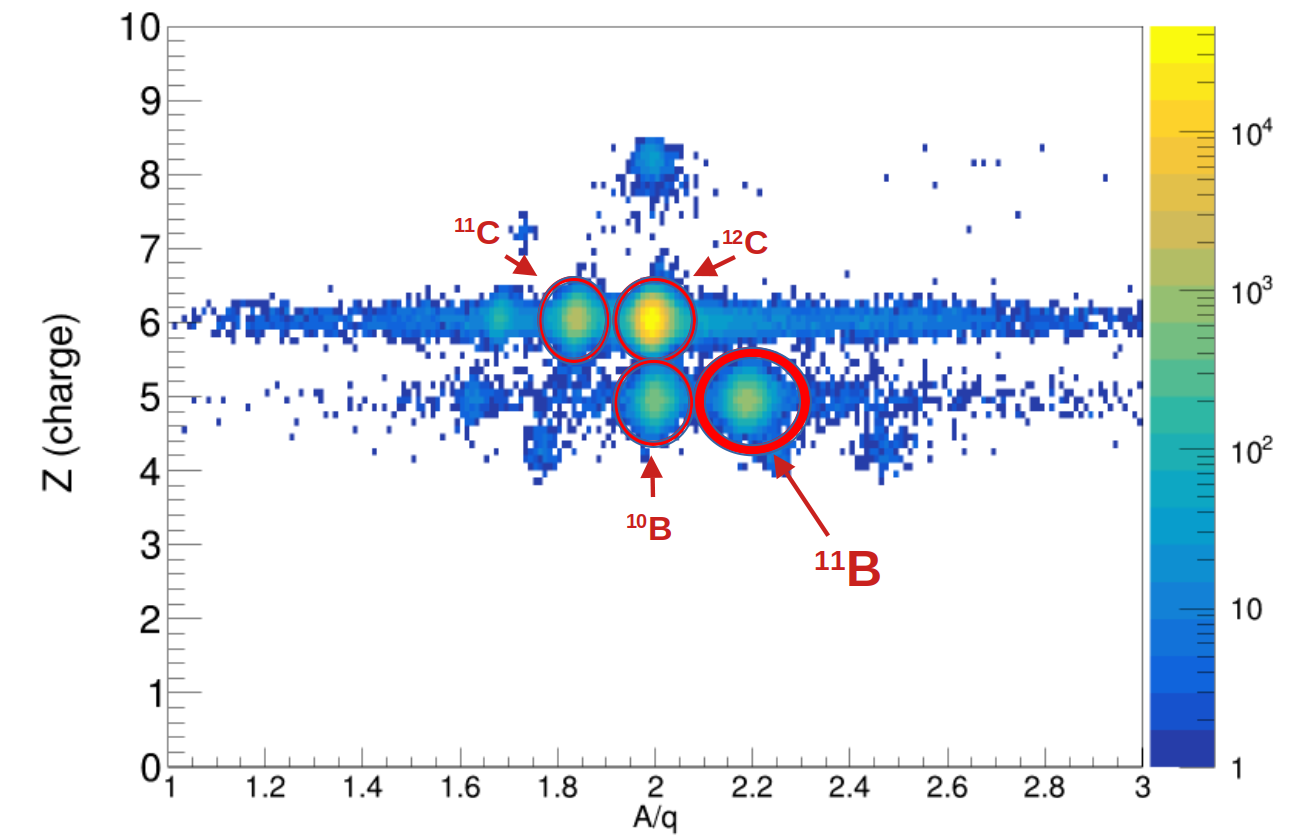
\includegraphics[width=\textwidth,height=12cm,keepaspectratio=true]{Figures/a_over_q_vs_q_plot.png}
    \caption{
	Fragment identification is performed using the correlation between the atomic number $Z$ and the mass-to-charge ratio $\frac{A}{q}$. For the quasi-free scattering (QFS) analysis of the reaction $^{12}C(p,2p)^{11}B$, the fragment of interest is $^{11}B$, which is emphasized with a bold red circle.
    }
    \label{fig:a_q_vs_q}
\end{figure}
For this qualitative analysis, the upper charge bound of $^{11}B$ was determined by locating the intersection point of the Gaussian-fitted distributions corresponding to the $Z=5$ and $Z=6$ peaks. The lower bound was set by applying an offset of minus one unit.\newline
A similar approach was employed to select the specific boron isotope $^{11}B$. The charge selection was performed using the previously defined boundary cuts. To isolate the $^{11}B$ isotopes, the lower bound was determined by identifying the intersection point of the Gaussian-fitted distributions corresponding to the $^{10}B$ and $^{11}B$ peaks. The upper bound was established by measuring the distance from this intersection point to the peak of $^{11}B$.

\subsection{QFS-Protons}\label{sec:qfs_protons}
Following the identification of the fragments through precise flight path reconstruction and time measurement, as detailed in the previous subsection, and the subsequent selection of the $^{11}B$ isotope, the analysis focuses on the two correlated protons to fully characterize the quasi-free scattering channel $^{12}C(p,2p)^{11}B$.\newline
For a proper interpretation of the data, it is essential to consider the geometric acceptance of CALIFA during the S444 experiment in 2020. The central \textit{BARREL} region (Ring 3 and Ring 4), covering the polar angular range from $43^{\circ}$ to $88^{\circ}$, was fully operational. In contrast, the forward region, referred to as \textit{iPhos} ($19^{\circ}$ to $43^{\circ}$), was only partially equipped, with a coverage of approximately $35\%$. The forward endcap, known as \textit{CEPA}, was not installed, and the backward barrel remained unoccupied. The corresponding geometry is illustrated in figure \ref{fig:qfs_reac_and_geo}.\newline
\begin{figure}[htpb]
	\begin{subfigure}[t]{.4\linewidth}
    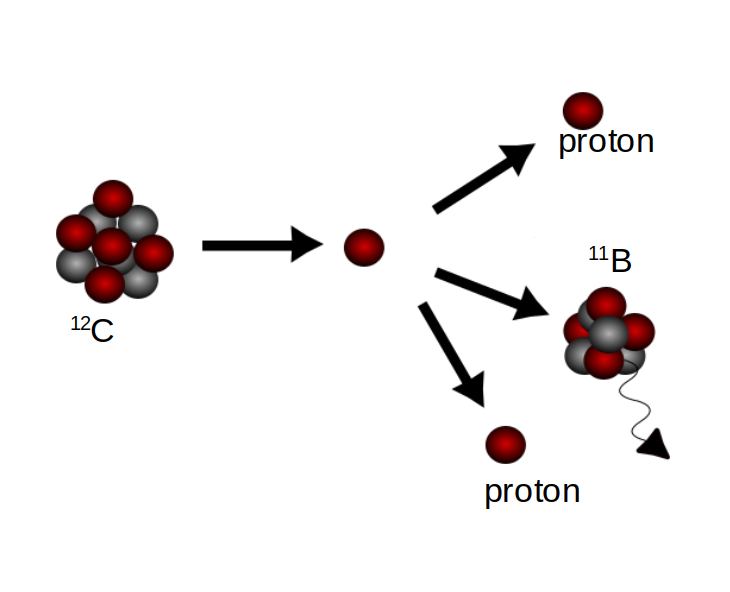
\includegraphics[width=\textwidth]{Figures/reaction_qfs_model.png}
	\caption{Quasi-free scattering channel $^{12}C(p,2p)^{11}B$}
	\end{subfigure}
	\begin{subfigure}[t]{.4\linewidth}
    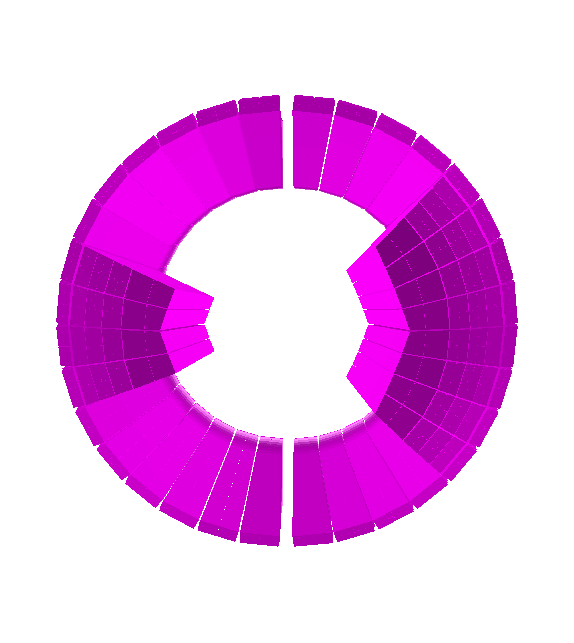
\includegraphics[width=\textwidth]{Figures/CALIFA2020Front.png}
	\caption{Simulated front view of the CALIFA calorimeter in 2020.}
	\end{subfigure}
    \caption{Tagging the $^{12}C(p,2p)^{11}B$ channel with only partly filled CALIFA calorimeter for the detection of the two correlated protons.}%
    \label{fig:qfs_reac_and_geo}%
\end{figure}
For the proton selection and the application of reasonable cuts it is important to understand the processing steps of the raw \textit{mapped} level data to the \textit{cal} level and finally \textit{hit} level data. The \textit{mapped} level data has following structure for each CALIFA hit:
For an accurate proton selection and the application of appropriate cuts, it is crucial to understand the data processing steps from the raw \textit{mapped}-level to the \textit{cal}-level and finally to the \textit{hit}-level. The \textit{mapped}-level data for each CALIFA hit is structured as follows:
\begin{itemize}
\item[$\blacksquare$] CrystalID: each crystal channel gets assigned a unique ID. Gamma range channels are in the range up to 2550, proton range ones from 2550 up to ..
\item[$\blacksquare$] Uncalibrated Energy
\item[$\blacksquare$] Slow Component $N_s$, extracted from the signal shape, see \cite{winkel2011implementierung}, section 2.
\item[$\blacksquare$] Fast Component $N_f$, extracted from the signal shape, see \cite{winkel2011implementierung}, section 2.
\item[$\blacksquare$] WRTS: White Rabbit Time Stamp\cite{serrano2013white}, interpolated from FEBEX inner clock.
\item[$\blacksquare$] Time over Threshold, optionally activated for $\gamma$-range channels to reconstruct energies beyond range.
\end{itemize}

The \textit{cal}-level data is structured as in the \textit{mapped}-level, however with calibrated energy by applying the calibration parameters from calibration run to each crystal channel.\newline
For the calibration runs a $^{22}Na$ (with peaks at $511keV$ and $1275keV$) or a $^{60}Co$ (with peaks at $1173keV$ and $1332keV$) source is used. For each crystal channel a linear fit on the two photopeaks is performed. Using this fitting function, the uncalibrated energy, expressed in energy channels, can be converted into calibrated energy values.\newline
For the final \textit{hit}-level data, the energy-calibrated hits from the \textit{cal}-level are merged into clusters. High-energy proton hits ($E_{hit} > 15 MeV$) and low-energy $\gamma$ hits are first listed and sorted in descending energy order. Clusters are then formed using a cone-shaped approach, where each cluster is centered around the highest-energy hit with a half-opening angle of $\theta_c = 14.3^{\circ}$. All hits within this angular region are merged into the cluster. This process is iteratively repeated until both the high- and low-energy lists are empty. To improve the signal-to-noise ratio in this analysis, hits with energy values below the threshold of $E_{thr} = 100keV$ are discarded during clustering.\newline
The resulting correlations in azimuthal and polar angles,with the only cut to have at least two high energy clusters with energy larger 15 MeV, with respect to the simulated \textit{p2p}-simulations are shown in figure \ref{fig:azimuth_corr} and figure \ref{fig:polar_corr} accordingly.\newline
\begin{figure}[htpb]
	\begin{subfigure}[t]{.75\linewidth}
    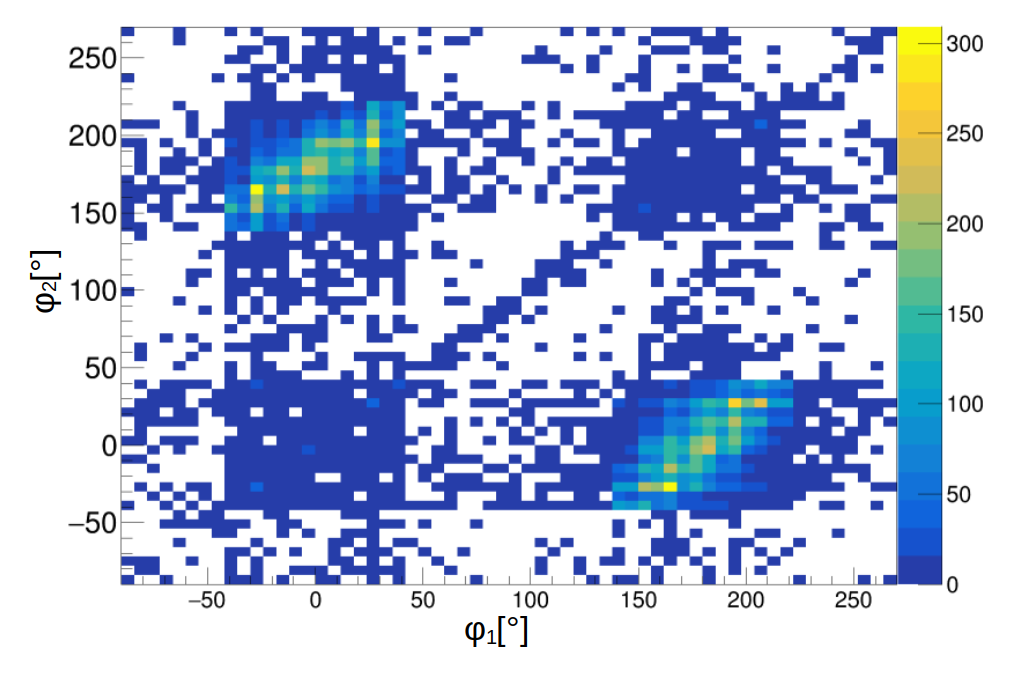
\includegraphics[width=\textwidth]{Figures/phi12_califa.png}
	\caption{Correlation from S444 experimental data}
	\end{subfigure}
	\begin{subfigure}[t]{.75\linewidth}
    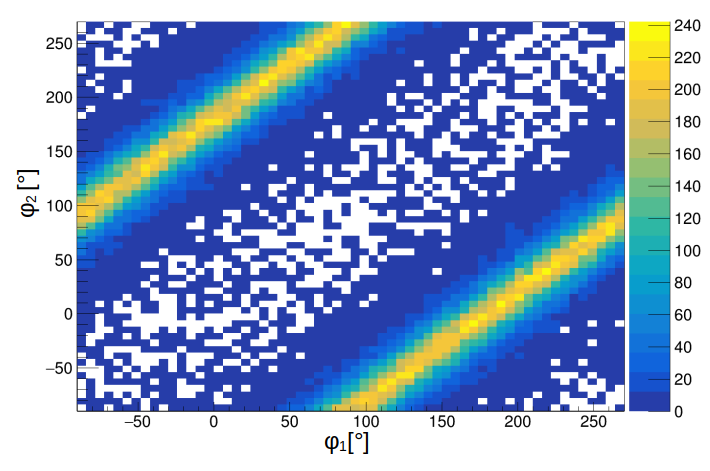
\includegraphics[width=\textwidth]{Figures/phi12_sim.png}
	\caption{Simulated data using based on QFS kinematical code by Leonid Chulkov, GSI.}
	\end{subfigure}
    \caption{Azimuthal angular correlation $\varphi_1$ versus $\varphi_2$ of the two clusters with highest energy in CALIFA }
    \label{fig:azimuth_corr}
\end{figure}
From the azimuthal correlation plot in Figure \ref{fig:azimuth_corr}, the geometric acceptance limitations of CALIFA become evident. In the so-called \textit{iPhos} region, CALIFA was instrumented only within the azimuthal ranges of $\pm 45^{\circ}$ and $157.5^{\circ}$ to $202.5^{\circ}$. Due to relativistic kinematics, both protons undergo a forward boost, leading to their predominant detection in the iPhos array. Consequently, any acceptance loss in this region has a substantial impact on the overall detection efficiency.\newline
Moreover, the correlation plot exhibits a distinct correlation line at $\varphi_1 \approx \varphi_2$. This feature primarily arises from inaccuracies in cluster reconstruction, where proton cluster hits fall outside the predefined cone size of the reconstruction algorithm, resulting in the erroneous identification of two separate hits. This effect is particularly pronounced in the \textit{iPhos} region as it is the primary detection region for the protons. Such misidentified events are systematically excluded in analyses focusing on the clean $^{12}C(p,2p)^{11}B$ channel.\newline
\begin{figure}[htpb]
	\begin{subfigure}[t]{.75\linewidth}
    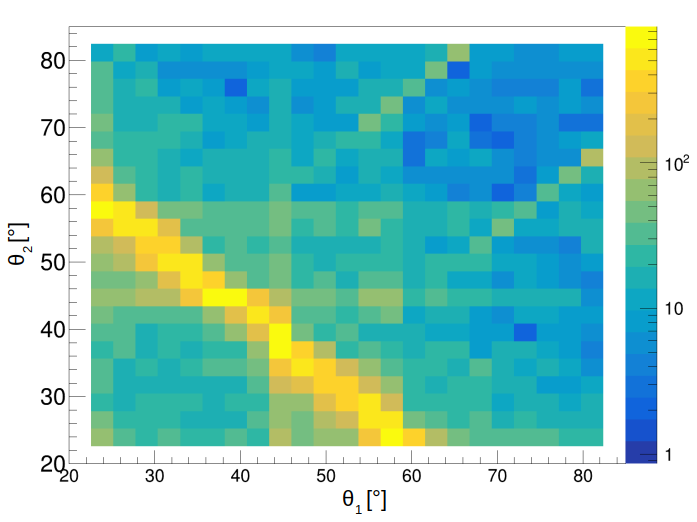
\includegraphics[width=\textwidth]{Figures/theta12_califa.png}
	\caption{Correlation from S444 experimental data}
	\end{subfigure}
	\begin{subfigure}[t]{.75\linewidth}
    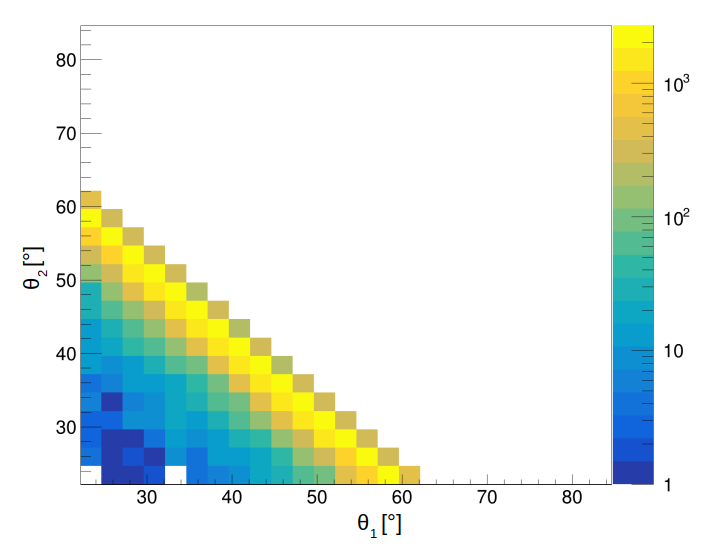
\includegraphics[width=\textwidth]{Figures/theta12_sim.png}
	\caption{Simulated data using based on QFS kinematical code by Leonid Chulkov, GSI.}
	\end{subfigure}
    \caption{Polar angular correlation $\theta_1$ versus $\theta_2$ of the two clusters with highest energy in CALIFA }
    \label{fig:polar_corr}
\end{figure}
The polar angular correlation in figure \ref{fig:polar_corr} shows as expected a strong anti-correlation between the two proton clusters. For beam energies up to approximately $500 AMeV$ the anti-correlation line is expected to be uniformly distributed over the polar range as the momentum transfer $t = -Q^2$, which defines the angular distributions $\theta_{1/2}$, does not effect the cross section in this energy regime\footnote{At higher beam energies, parameterizations of the cross section as a function of $t$ often take the form $\frac{d\sigma}{dt} = C e^{bt}$, where $C$ and $b$ are empirically determined parameters.}.\newline
Moreover in figure \ref{fig:polar_corr} the two off-diagonal lines should be noted. This artifact arises from wrong cluster reconstruction where proton cluster hits fall outside the predefined cone size of the reconstruction algorithm, resulting in the erroneous identification of two separate hits. As the resulting clusters are in close proximity, they exhibit a systematic offset from the diagonal in the polar angular correlation plot.\newline
The information of azimuthal and polar angles of the two protons can merged in the opening angle of the two reconstructed protons via the geometric formula:
\begin{equation}\label{eq:opang}
\theta_{p2p} = acos\left( \sin(\theta_1) \sin(\theta_2) \cos(\varphi_2 - \varphi_1) + \cos(\theta_1) \cos(\theta_2) \right)
\end{equation}

\begin{figure}[htpb]
	\begin{subfigure}[t]{.43\linewidth}
    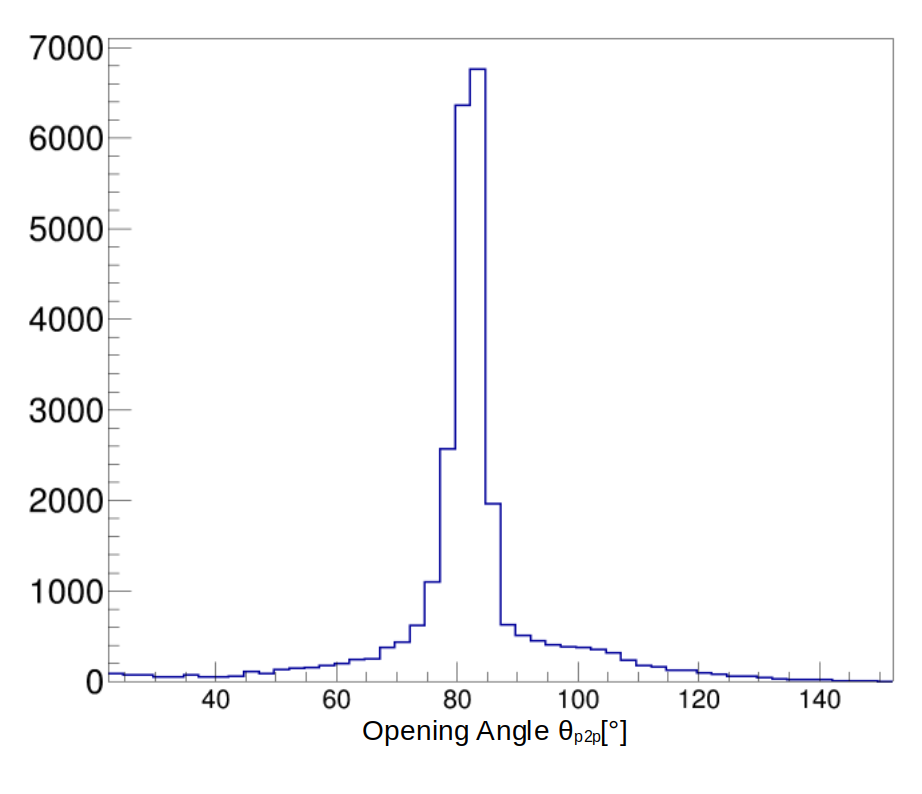
\includegraphics[width=\textwidth]{Figures/opang.png}
	\caption{Opening angle distribution from S444 experimental data}
	\end{subfigure}
	\begin{subfigure}[t]{.47\linewidth}
    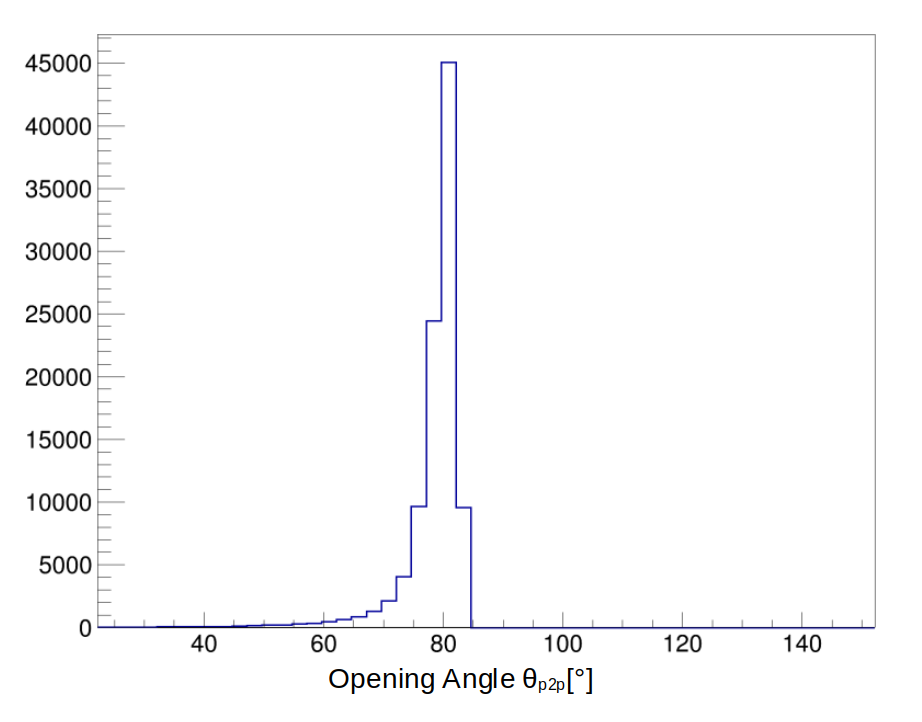
\includegraphics[width=\textwidth]{Figures/opang_sim.png}
	\caption{Simulated opening angle $\theta_{p2p}$ based on QFS kinematical code by Leonid Chulkov, GSI.}
	\end{subfigure}
    \caption{Reconstruction of the opening angle $\theta_{p2p}$ as in equation \ref{eq:opang} from the two clusters with highest energy in CALIFA }
    \label{fig:opang}
\end{figure}

Figure \ref{fig:opang} presents the opening angle $\theta_{p2p}$ for the reconstructed protons. In both the simulated and experimental data, the distribution exhibits a peak at approximately $81^{\circ}$. While the simulated distribution shows a strict upper limit around $82^{\circ}$, the experimental data features a pronounced tail extending toward larger values. This effect is primarily attributed to final-state interactions (FSI) and can be significantly reduced by applying appropriate selection criteria to the polar and azimuthal angular correlations of the two reconstructed high-energy hits.\newline
Herefore in the next considerations only events with following criteria are selected:
\begin{itemize}
\item $\theta_1 + \theta_1 < 90^{\circ}$
\item $\Delta \varphi < 180 \pm 40^{\circ}$
\end{itemize}

\subsubsection{Missing Momentum $\mathbf{p_{miss}}$ Reconstruction}\label{sec:p_miss}

As discussed in Section \ref{sec:qfs_theo}, the momentum of the knocked-out proton inside the $^{12}C$ nucleus can be reconstructed, assuming higher-order perturbations are negligible, as described by Equation \ref{eq:miss_mom}. For this reconstruction, the momenta of the two detected protons, $\mathbf{p_{1/2}}$, and the initial target proton, $\mathbf{p_{0}}$ (which is approximately zero in the laboratory frame), must be known and transformed into the center-of-mass frame of the $^{12}C$ nucleus. The resulting distribution of the missing momentum, $\mathbf{p_{miss}}$, obtained from experimental data, is presented in Figure \ref{fig:p_miss}.\newline
\begin{figure}[htpb]
    \centering
    % Large subfigure
    \begin{subfigure}[b]{0.9\textwidth}
        \centering
        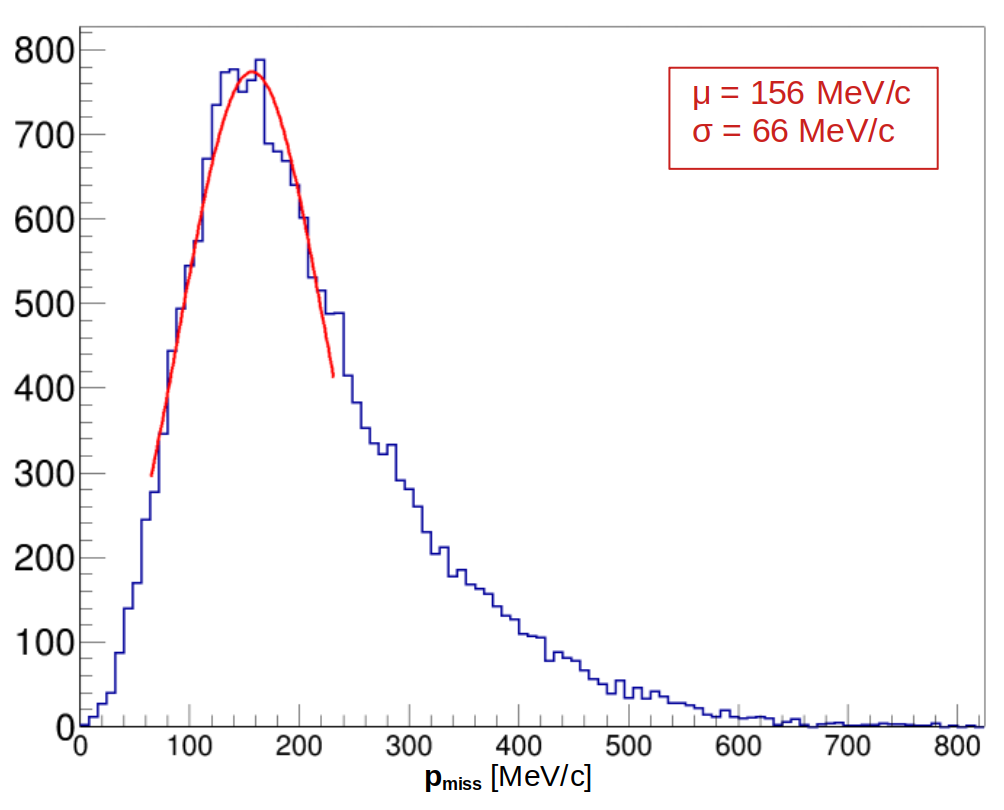
\includegraphics[width=\textwidth]{Figures/p_miss_tot.png} % Replace with your image file
        \caption{Reconstructed absolulte value of $\mathbf{p_{miss}}$.}
        \label{fig:p_miss_tot}
    \end{subfigure}

    % Row of three smaller subfigures
    \begin{subfigure}[b]{0.3\textwidth}
        \centering
        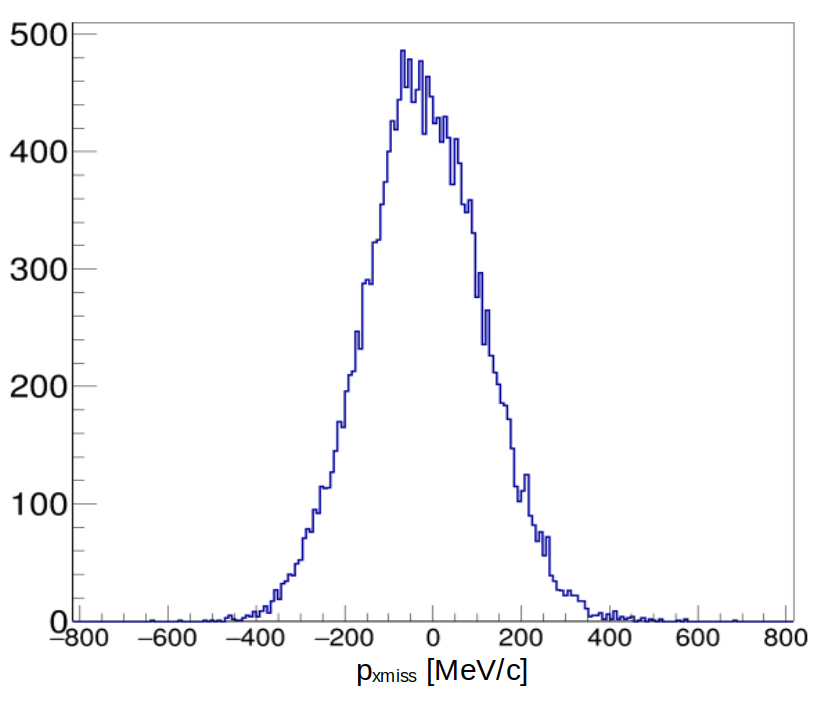
\includegraphics[width=\textwidth]{Figures/p_miss_x.png} % Replace with your image file
        \caption{Reconstructed\newline x-component of $\mathbf{p_{miss}}$.}
        \label{fig:p_miss_x}
    \end{subfigure}
    \begin{subfigure}[b]{0.3\textwidth}
        \centering
        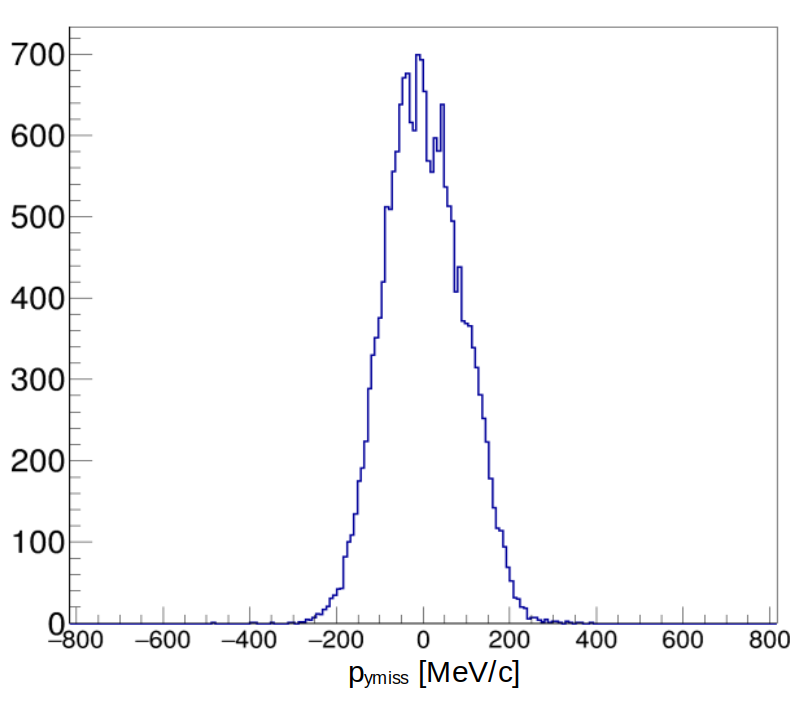
\includegraphics[width=\textwidth]{Figures/p_miss_y.png} % Replace with your image file
        \caption{Reconstructed\newline y-component of $\mathbf{p_{miss}}$.}
        \label{fig:p_miss_y}
    \end{subfigure}
    \begin{subfigure}[b]{0.3\textwidth}
        \centering
        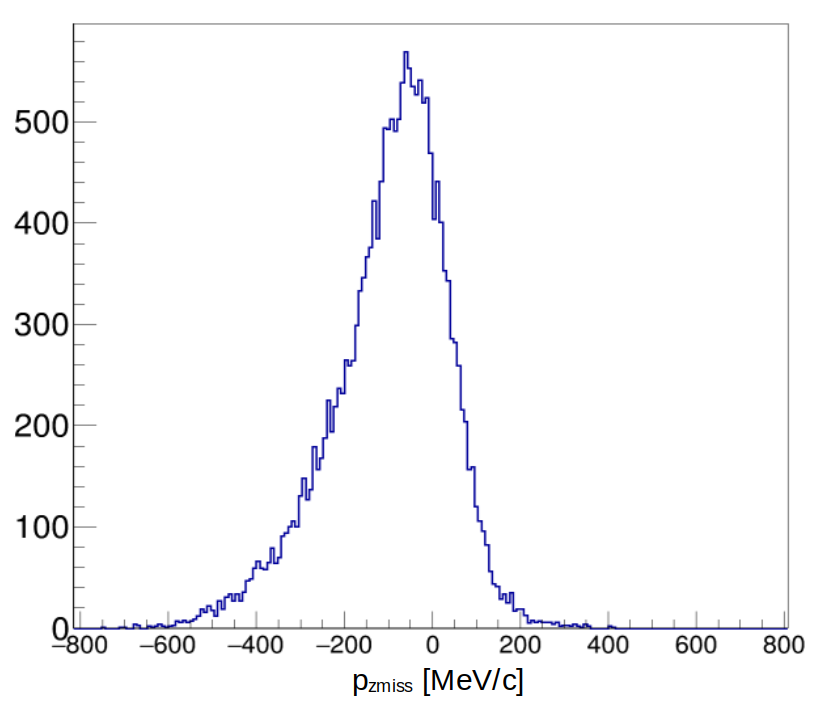
\includegraphics[width=\textwidth]{Figures/p_miss_z.png} % Replace with your image file
        \caption{Reconstructed\newline z-component of $\mathbf{p_{miss}}$.}
        \label{fig:p_miss_z}
    \end{subfigure}

    \caption{Reconstructed $\mathbf{p_{miss}}$ and its components in the $^{12}C$ rest frame}
    \label{fig:p_miss}
\end{figure}

Compared to previous experimental results, such as those reported in Ref. \cite{moniz1971nuclear}, where the measured Fermi momentum for $^{12}C$ was determined to be $221 \mp 5$ MeV/c, corresponding to a mean internal proton momentum of $171$ MeV/c, the reconstructed mean value in the present analysis is found to be $156$ MeV/c.\newline
While this value is slightly lower than the reference, it is important to consider the specific experimental conditions. The geometric acceptance of CALIFA, particularly in the forward region, was not fully instrumented, which may introduce some distortions in the reconstructed $\mathbf{p_{miss}}$ distribution. Nevertheless, the obtained results remain consistent within the expected systematic uncertainties.\newline
Furthermore, the beam energy, assumed to be constant at $400, A\text{MeV}$, plays a crucial role in transforming the reconstructed proton momenta into the center-of-mass frame of the $^{12}C$ nucleus. Small variations in the actual beam energy could have a non-negligible impact on the missing momentum reconstruction. Since no precise event-by-event beam energy information was available for this analysis, a constant value of $400$ AMeV was used.\newline
Additionally, as shown in Figure \ref{fig:p_miss_z}, the distribution of the z-component of $\mathbf{p_{miss}}$ exhibits a slight asymmetry, with a tail extending toward lower values. Since the z-component is particularly sensitive to deviations in the mean beam energy, this effect further contributes to the shift of the mean $\mathbf{p_{miss}}$ value toward lower values. Future studies with improved acceptance corrections and access to event-wise beam energy measurements could further refine the results and enhance the accuracy of the $\mathbf{p_{miss}}$ reconstruction.


\subsubsection{Correlations between $^{11}B$ Fragment and the reconstructed inner Proton }
%In subsection \ref{sec:p_miss} we reconstructed the momentum of the inner proton $\mathbf{p_{miss}}$. Herefore only data from the CALIFA calorimeter was necessary. As next step the reconstructed inner proton momentum $\mathbf{p_{miss}}$ can be correlated with the reconstructed $^{11}B$ momentum in the $^{12}C$ rest frame. The momenta of the two constituents of the $^{12}C$, the reconstruced proton and the $^{11}B$, should add up to zero since this is the definition of the rest frame. That means that the momentum vectors of the inner proton and the $^{11}B$ accordingly should point to opposite directions. Which again means for the cosine of the angle $\gamma$ between the two constituents should be approximately -1. This is also what we receive from data, as shown in figure \ref{fig:cos_gamma}.\newline
%Moreover figure \ref{fig:x_corr_p_miss_11b} and \ref{fig:y_corr_p_miss_11b} show the correlation between the x and y momentum of the inner proton to the accoring component of the $^{11}B$ accordingly. In both cases a strong anti-correlation is visible. While the correlation plot for the y component is relatively sharp, the one for the x component is quite blurred. This really comes from the geometric dependent resolutions in the subdetectors:\newline
%For the x component it has to be considered that only the side halves of CALIFA are filled in the \textit{iPhos} region ($\varphi_{1/2}$ in the region $\pm 45^{\circ}$ and $157.5^{\circ}$ to $202.5^{\circ}$). The angular resolution in $\varphi$ is only moderate ($\approx \frac{6^{\circ}}{sqrt{12}}$ and the x component reconstruction is proportional to $\cos(\varphi)$ with an only slowly changing derivative ($\sin(\varphi)$) for $\varphi \approx 0$. Moreover the x component of the $^{11}B$ fragment has to be reconstructed from the position resolutions right after the target with a small lever arm compared to the reconstruction of the y component of the $^{11}B$ fragment which is reconstructed from the y information in MWCP3 after GLAD, since the y component should not be affected by the GLAD magnet. 
%
In Subsection \ref{sec:p_miss}, the momentum of the inner proton, $\mathbf{p_{miss}}$, was reconstructed using data exclusively from the CALIFA calorimeter. As a next step, this reconstructed momentum can be correlated with the momentum of the $^{11}B$ fragment in the rest frame of the $^{12}C$ nucleus.\newline

Since the total momentum in the rest frame must be zero by definition, the momentum vectors of the inner proton and the $^{11}B$ fragment should be directed oppositely. Consequently, the cosine of the angle $\gamma$ between these two constituents should be approximately $-1$, which is confirmed by the experimental data, as shown in Figure \ref{fig:cos_gamma}.\newline

Furthermore, Figures \ref{fig:x_corr_p_miss_11b} and \ref{fig:y_corr_p_miss_11b} illustrate the correlation between the x- and y-components of $\mathbf{p_{miss}}$ and the corresponding components of the $^{11}B$ fragment. A strong anti-correlation is observed in both cases. While the correlation in the y-component is relatively sharp, the x-component exhibits a more blurred distribution.\newline

This effect arises from the geometry-dependent resolution of the subdetectors:
\begin{itemize}
\item[--]For the x-component, it is important to consider that only the lateral halves of CALIFA were instrumented in the \textit{iPhos} region ($\varphi_{1/2}$ within $\pm 45^{\circ}$ and $157.5^{\circ}$ to $202.5^{\circ}$). The azimuthal resolution is moderate ($\approx \frac{6^{\circ}}{\sqrt{12}}$), and since the x-component is reconstructed as $\propto \cos(\varphi)$, the derivative $\sin(\varphi)$ remains small for $\varphi \approx 0$, leading to lower sensitivity in this region.
\item[--] The x-component of the $^{11}B$ fragment is reconstructed from position measurements immediately after the target, where the lever arm for momentum reconstruction is relatively short.
\item[--]In contrast, the y-component of the $^{11}B$ fragment is determined from its position in MWPC3 after GLAD, where the larger lever arm improves resolution. Moreover, the y-component remains largely unaffected by the GLAD magnet, further enhancing its reconstruction accuracy.
\end{itemize}

\begin{figure}[!htb]
    \centering
    % Large subfigure on the left
    \begin{subfigure}[b]{0.9\textwidth}
        \centering
        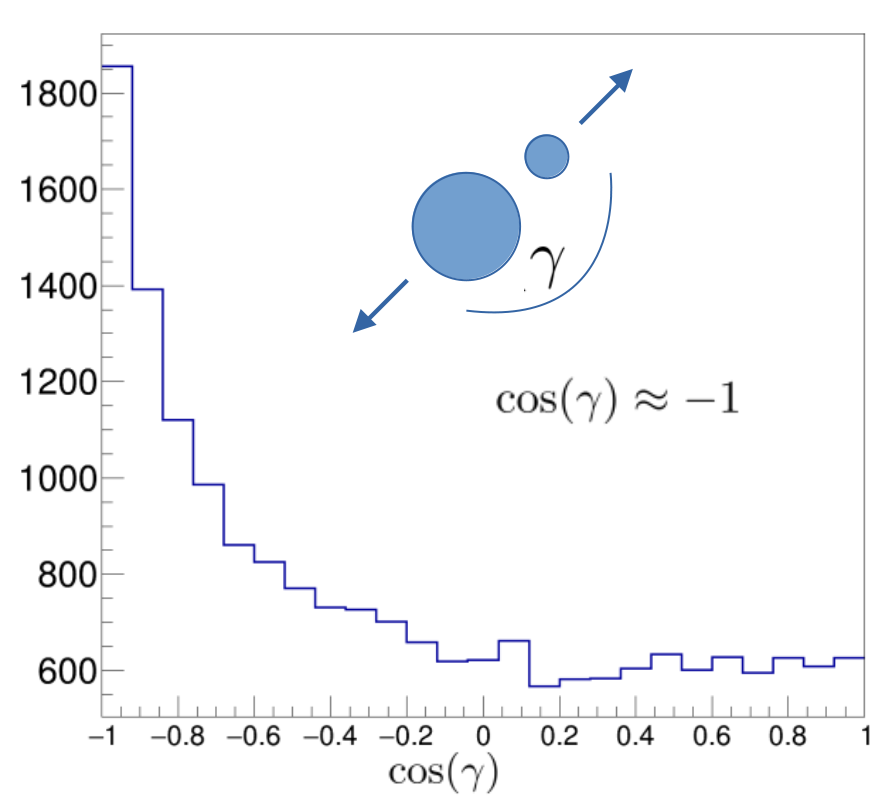
\includegraphics[width=\textwidth]{Figures/cos_angle_2p_11b.png} % Replace with actual image
        \caption{Cosine of the angle $\gamma$ between inner proton and $^{11}B$.}
        \label{fig:cos_gamma}
    \end{subfigure}

    \vspace{0.3cm} % Adjust vertical spacing

    % Row for two smaller subfigures
    \begin{subfigure}[b]{0.39\textwidth}
        \centering
        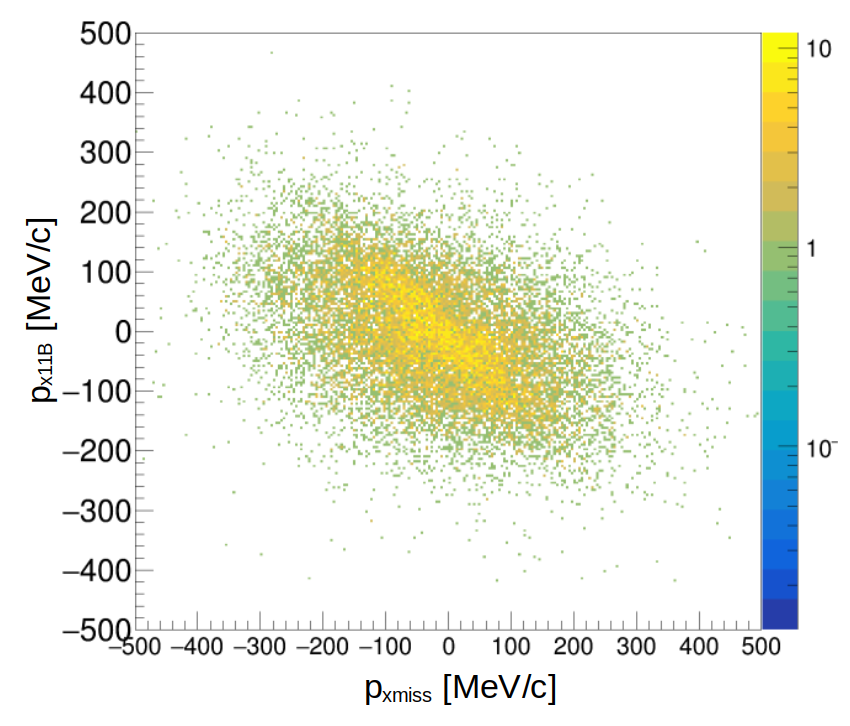
\includegraphics[width=\textwidth]{Figures/p_x_2p_11b.png} % Replace with actual image
        \caption{x-component correlation between inner proton and $^{11}B$.}
        \label{fig:x_corr_p_miss_11b}
    \end{subfigure}
    \hspace{0.2cm} % Adjust horizontal spacing
    \begin{subfigure}[b]{0.39\textwidth}
        \centering
        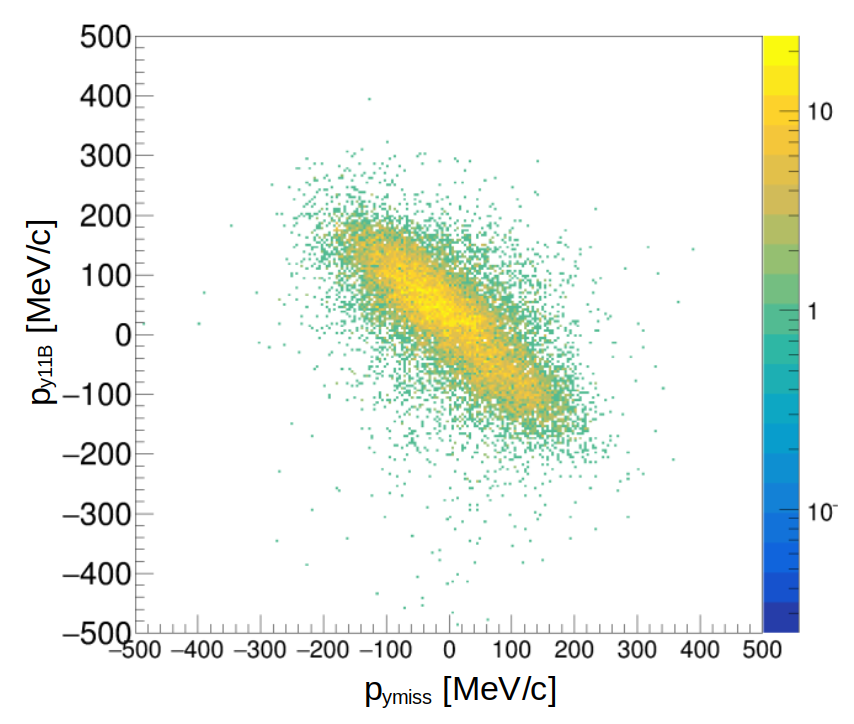
\includegraphics[width=\textwidth]{Figures/p_y_2p_11b.png} % Replace with actual image
        \caption{y-component correlation between inner proton and $^{11}B$.}
        \label{fig:y_corr_p_miss_11b}
    \end{subfigure}

    %% Small subfigures stacked on the right
    %\begin{subfigure}[b]{0.9\textwidth}
    %    \centering
    %    \begin{subfigure}[b]{0.9\textwidth}
    %        \centering
    %        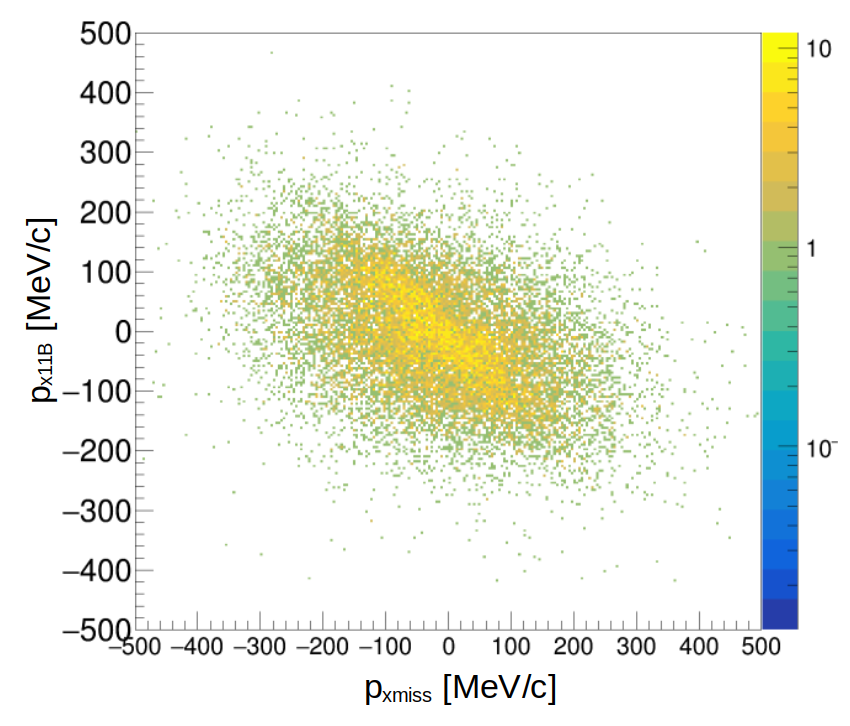
\includegraphics[width=0.45\textwidth]{Figures/p_x_2p_11b.png} % Replace with actual image
    %        \caption{x-component correlation between inner proton and $^{11}B$.}
    %        \label{fig:x_corr_p_miss_11b}
    %    \end{subfigure}
    %    \vspace{0.2cm}
    %    \begin{subfigure}[b]{0.9\textwidth}
    %        \centering
    %        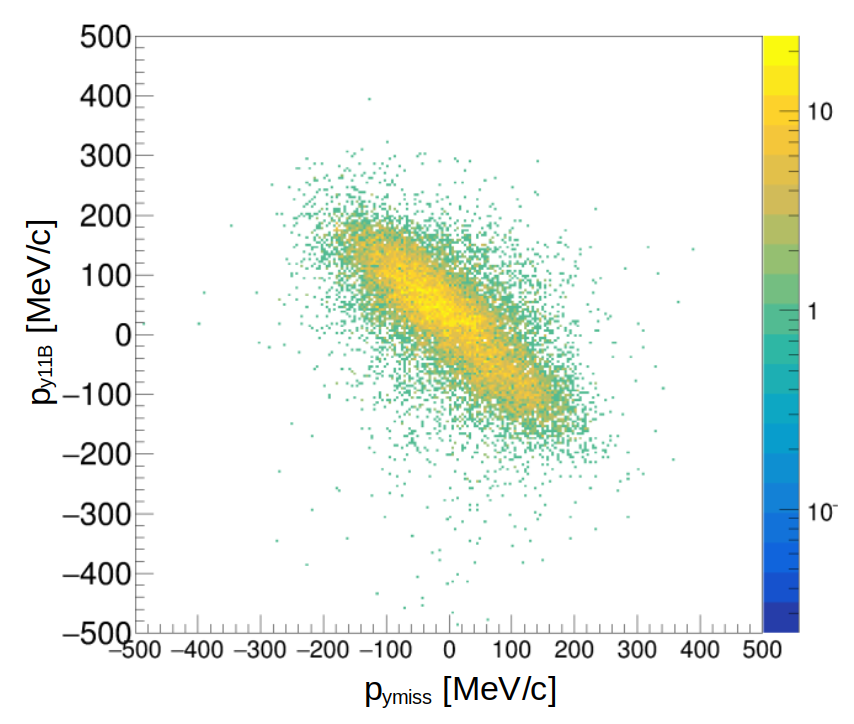
\includegraphics[width=0.45\textwidth]{Figures/p_y_2p_11b.png} % Replace with actual image
    %        \caption{y-component correlation between inner proton and $^{11}B$.}
    %        \label{fig:y_corr_p_miss_11b}
    %    \end{subfigure}
    %\end{subfigure}
    
    \caption{Correlation plots between inner proton and $^{11}B$ in the $^{12}C$ rest frame.}
    \label{fig:corr_p_miss_11b}
\end{figure}

TODO:->Maybe also correlations between fragment and proton pair, see Chulkov.


\subsubsection{Proton Separation Energy $S_p$}
The proton separation energy $S_p$ of $^{12}C$ from the reaction channel $^{12}C(p,2p)^{11}B$ is defined by the masses and energies of the initial and final state particles in the $^{12}C$ rest frame. One can write the full energy conservation in the rest frame of $^{12}C$:
\begin{equation}
M_{^{12}C} + \gamma \cdot m_p = E_1^* + E_2^* + (M_{^{11}B} + E_{ex})  + T_{^{11}B^*}
\end{equation}
where $E_1^*$ and $E_2^*$ are total energies of the two protons in the $^{12}C$ rest frame, $E_{ex}$ is residual excitation in $^{11}B$ and $T_{^{11}B^*}$ the kinetic energy of the $^{11}B$ in the $^{12}C$ rest frame.\newline
Using this equation, one can express the total binding energy $B$ of the knocked out nucleon:
\begin{equation}
B = S_p - E_{ex} = M_{^{12}C} - M_{^{11}B} - E_{ex} - m_p = E_1^* + E_2^* + T_{^{11}B^*} - \gamma \cdot m_p - m_p
\end{equation}
Using Lorentz transformation from lab to 12C rest frame one can obtain for $E_1^*/E_2^*$:
\begin{align*}
E_{1/2}^* &=  \gamma \cdot m_p + \gamma \cdot T_{1/2} - \beta \cdot \gamma \cdot p_{1/2} \cdot cos(\theta_{1/2})
\end{align*}
The kinetic energy of the $^{11}B$ in the $^{12}C$ rest frame can be written as:
\begin{align*}
T_{^{11}B^*} &= \frac{p_i^2}{2 \cdot M_{^{11}B}}
\end{align*}
with $p_i$ the inner momentum of the proton knocked out of the $^{12}C$ projectile, see equation \ref{eq:miss_mom}.
Putting this in the previous equation one finally gets for the binding energy $B$:
\begin{equation}
B = (\gamma - 1)\cdot m_p + \gamma \cdot (T_1+T_2) - \beta \cdot \gamma \cdot(p_1*cos(\theta_1) + p_2*cos(\theta_2)) + T_{^{11}B}
\end{equation}\label{eq:sep_energy}
For $E_{ex} = 0$, i.e. the fragment $^{11}B$ in the ground state, the binding energy $B$ is equal to the one proton separation energy $S_p$\footnote{Since the $^{11}B$ fragment predominantly remains in its ground state---implying that, in most cases, the outermost protons are removed---the binding energy $B$ and the proton separation energy $S_p$ are used interchangeably, also due to the limited energy resolution.}. \newline
As for the S444 experiment no target detector tracking system was available. Consequently the energies as well as the azimutal ($\varphi$) and polar($\theta$) angles of the two correlated protons had to be fully reconstructed using the CALIFA calorimeter. The calorimeter provided an energy resolution $\frac{\Delta E}{E}(@100MeV) \lesssim 1 \%$, along with angular resolutions of approximately  $\Delta \varphi \approx \frac{6^{\circ}}{\sqrt{12}}$, and $\Delta \theta \approx \frac{2^{\circ}}{\sqrt{12}}$.
The best way to visualize the separation energy $S_p$ id to plot it against the summed energy of the two protons in the $^{12}C$ rest frame as shown in figure \ref{fig:sep_energy}. Two vertical lines are visible. They correspond to the two QFS-reaction types within the $CH_2$ target: the proton within the $^{12}C$ projectile can either scatter on the hydrogen (proton-like) part of on the carbon part of the plastic target. For the first case only the separation energy $S_p$ as derived in equation \ref{eq:sep_energy} is necessary to remove the proton of the projectile within the $^{12}C$ nucleus. In the second case the QFS-reaction is between two protons both bound within a carbon nucleus -- the projectile carbon and the target carbon part. Herefore more energy is needed to free both protons from their nuclear bond. This corresponds to the left vertical line in figure \ref{fig:sep_energy}. It should be noted that the reconstructed one-proton separation energy $S_p$ is shifted with respect to the mean value of $\approx 16 MeV$. For a precise measurement the accurate position of the target and the reaction vertex would be needed, as well as a precise measurement of the kinetic energy of the incoming $^{12}C$ would be required (for the actual measurements the beam energy value was set to $400 AMeV$). 
\begin{figure}[htpb]
    \centering
    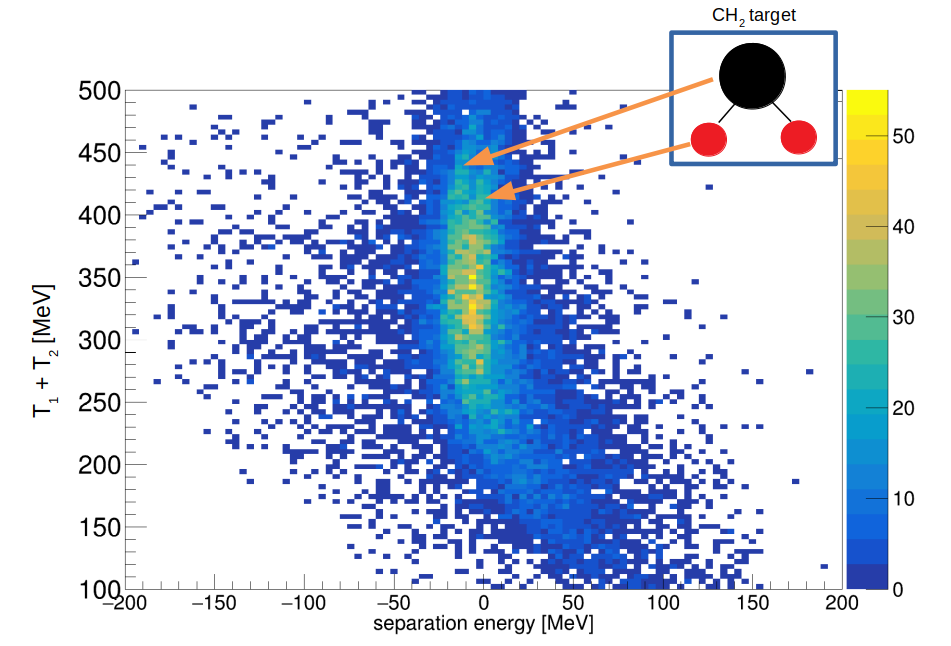
\includegraphics[width=\textwidth,height=10cm,keepaspectratio=true]{Figures/sep_energy_vs_sum_energy.png}
    \caption{
	Sum of the kinetic energies of the two correlated protons ($T_1/T_2$) versus the one proton separation energy $S_p$. Since this energy is needed to solve the proton from the nucleus' core, it's valuehas conventionally a negative sign.  	 
    }
    \label{fig:sep_energy}
\end{figure}

\subsection{Reconstruction of excited$ ^{11}$B states}
In order to achieve a complete kinematic reconstruction of the reaction products, the use of the CALIFA detector as a $\gamma$-ray spectrometer in the low-energy regime (down to $E_\gamma \geq 100\,\mathrm{keV}$) is essential. This is particularly relevant for reactions such as $^{12}\mathrm{C}(p,2p)^{11}\mathrm{B}$ in quasi-free scattering (QFS) kinematics. In such cases, it is possible to simultaneously identify and measure the energy of the two correlated protons (as demonstrated in previous sections) as well as detect $\gamma$-rays emitted during the de-excitation of $^{11}\mathrm{B}$ from excited states to its ground state ($3/2^-$).

$\gamma$-ray spectroscopy serves as a sensitive probe for investigating the population of low-lying discrete nuclear states. In the case of exotic nuclei, this allows exploration of previously uncharted excited states. For well-known nuclei such as $^{11}\mathrm{B}$, it provides an opportunity to test theoretical shell-model predictions and extract spectroscopic factors with high precision. The established level scheme of $^{11}\mathrm{B}$ is illustrated in Figure~\ref{fig:11B_levels}.
\begin{figure}[htpb]
    \centering
    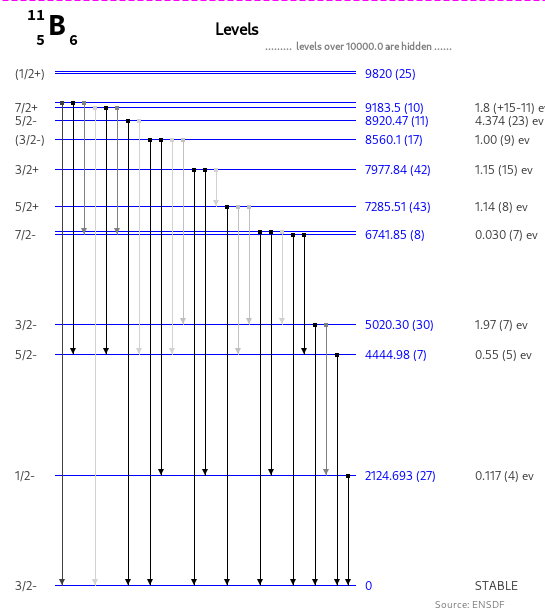
\includegraphics[width=\textwidth,height=8cm,keepaspectratio=true]{Figures/levelschemaplot.png}
    \caption{
Level scheme of $^{11}\mathrm{B}$ taken from~\cite{iaea_nuclide_chart}.
    }
    \label{fig:11B_levels}
\end{figure}

Assuming the ground-state proton configuration of $^{12}\mathrm{C}$ as $(s_{1/2})^2(p_{3/2})^4$, the removal of a single proton from the $p$-shell is expected to result in a hole state with quantum numbers corresponding to either $3/2^-$ or $1/2^-$. The population of higher angular momentum states is strongly suppressed due to the absence of significant contributions from indirect two-step processes and the limiting influence of ground-state correlations in $^{12}\mathrm{C}$~\cite{van1988weak}.

Some excited states of $^{11}\mathrm{B}$, such as the $5/2^-$ state with a known transition energy of 4.4~MeV, are not expected to be populated under QFS conditions. This state arises from the coupling of angular momenta of multiple unpaired nucleons (e.g., two nucleons in the $p_{3/2}$ orbital coupled to $J_{12} = 2$, and a third nucleon in $p_{1/2}$ with $J_3 = 1/2$). The population of such states via a QFS reaction would contradict the fundamental mechanism of QFS, which involves the interaction of the probe (typically a proton) with a single nucleon, while the remaining $A-1$ nucleons act as spectators.

As the $^{11}\mathrm{B}$ fragments produced in the reaction carry nearly the full beam energy and move predominantly in the forward direction, the emitted $\gamma$-rays from their de-excitation experience relativistic Doppler shifts. Therefore, Doppler correction must be applied to the measured $\gamma$-ray energies. Following standard textbooks (e.g.,~\cite{krane1987}), the relation between the observed $\gamma$-ray energy in the laboratory frame and the rest-frame energy of the emitting nucleus is given by:

\begin{equation}
    E_\gamma = E_0 \cdot \gamma \cdot (1 - \beta \cos \theta)
	\label{eq:doppler}
\end{equation}

where $E_0$ is the intrinsic $\gamma$-ray energy in the rest frame of $^{11}\mathrm{B}$ (approximately the same as the rest frame of the incoming $^{12}\mathrm{C}$), $\gamma = 1/\sqrt{1 - \beta^2}$ is the Lorentz factor, $\beta = v/c$ is the velocity of the $^{11}\mathrm{B}$ fragment normalized to the speed of light, and $\theta$ is the polar angle of the emitted $\gamma$-ray with respect to the beam axis in the laboratory frame\footnote{Since the excited state $1/2^-$ of $^{11}\mathrm{B}$ has a lifetime $T_{1/2} = 3.8$fs (which corresponds to a width of $\Gamma = 0.117$eV, see level scheme in Fig.~\ref{fig:11B_levels}) it is an immediate transition already occurring in the target region.}.\newline
The high granularity of the CALIFA calorimeter enables a precise determination of the emission angle $\theta$ of detected $\gamma$-rays. For each $\gamma$-ray event, the angle $\theta$ is defined by the position of the individual crystal within the $\gamma$-cluster that recorded the maximum deposited energy. This crystal is assumed to represent the most probable direction of the primary $\gamma$-ray emission. The angle is then used--relative to the known target position--to perform the Doppler correction and reconstruct the rest-frame $\gamma$-ray energy $E_0$, according to the relativistic transformation described in Eq.~\eqref{eq:doppler}.
\begin{figure}[htpb]
    \centering
    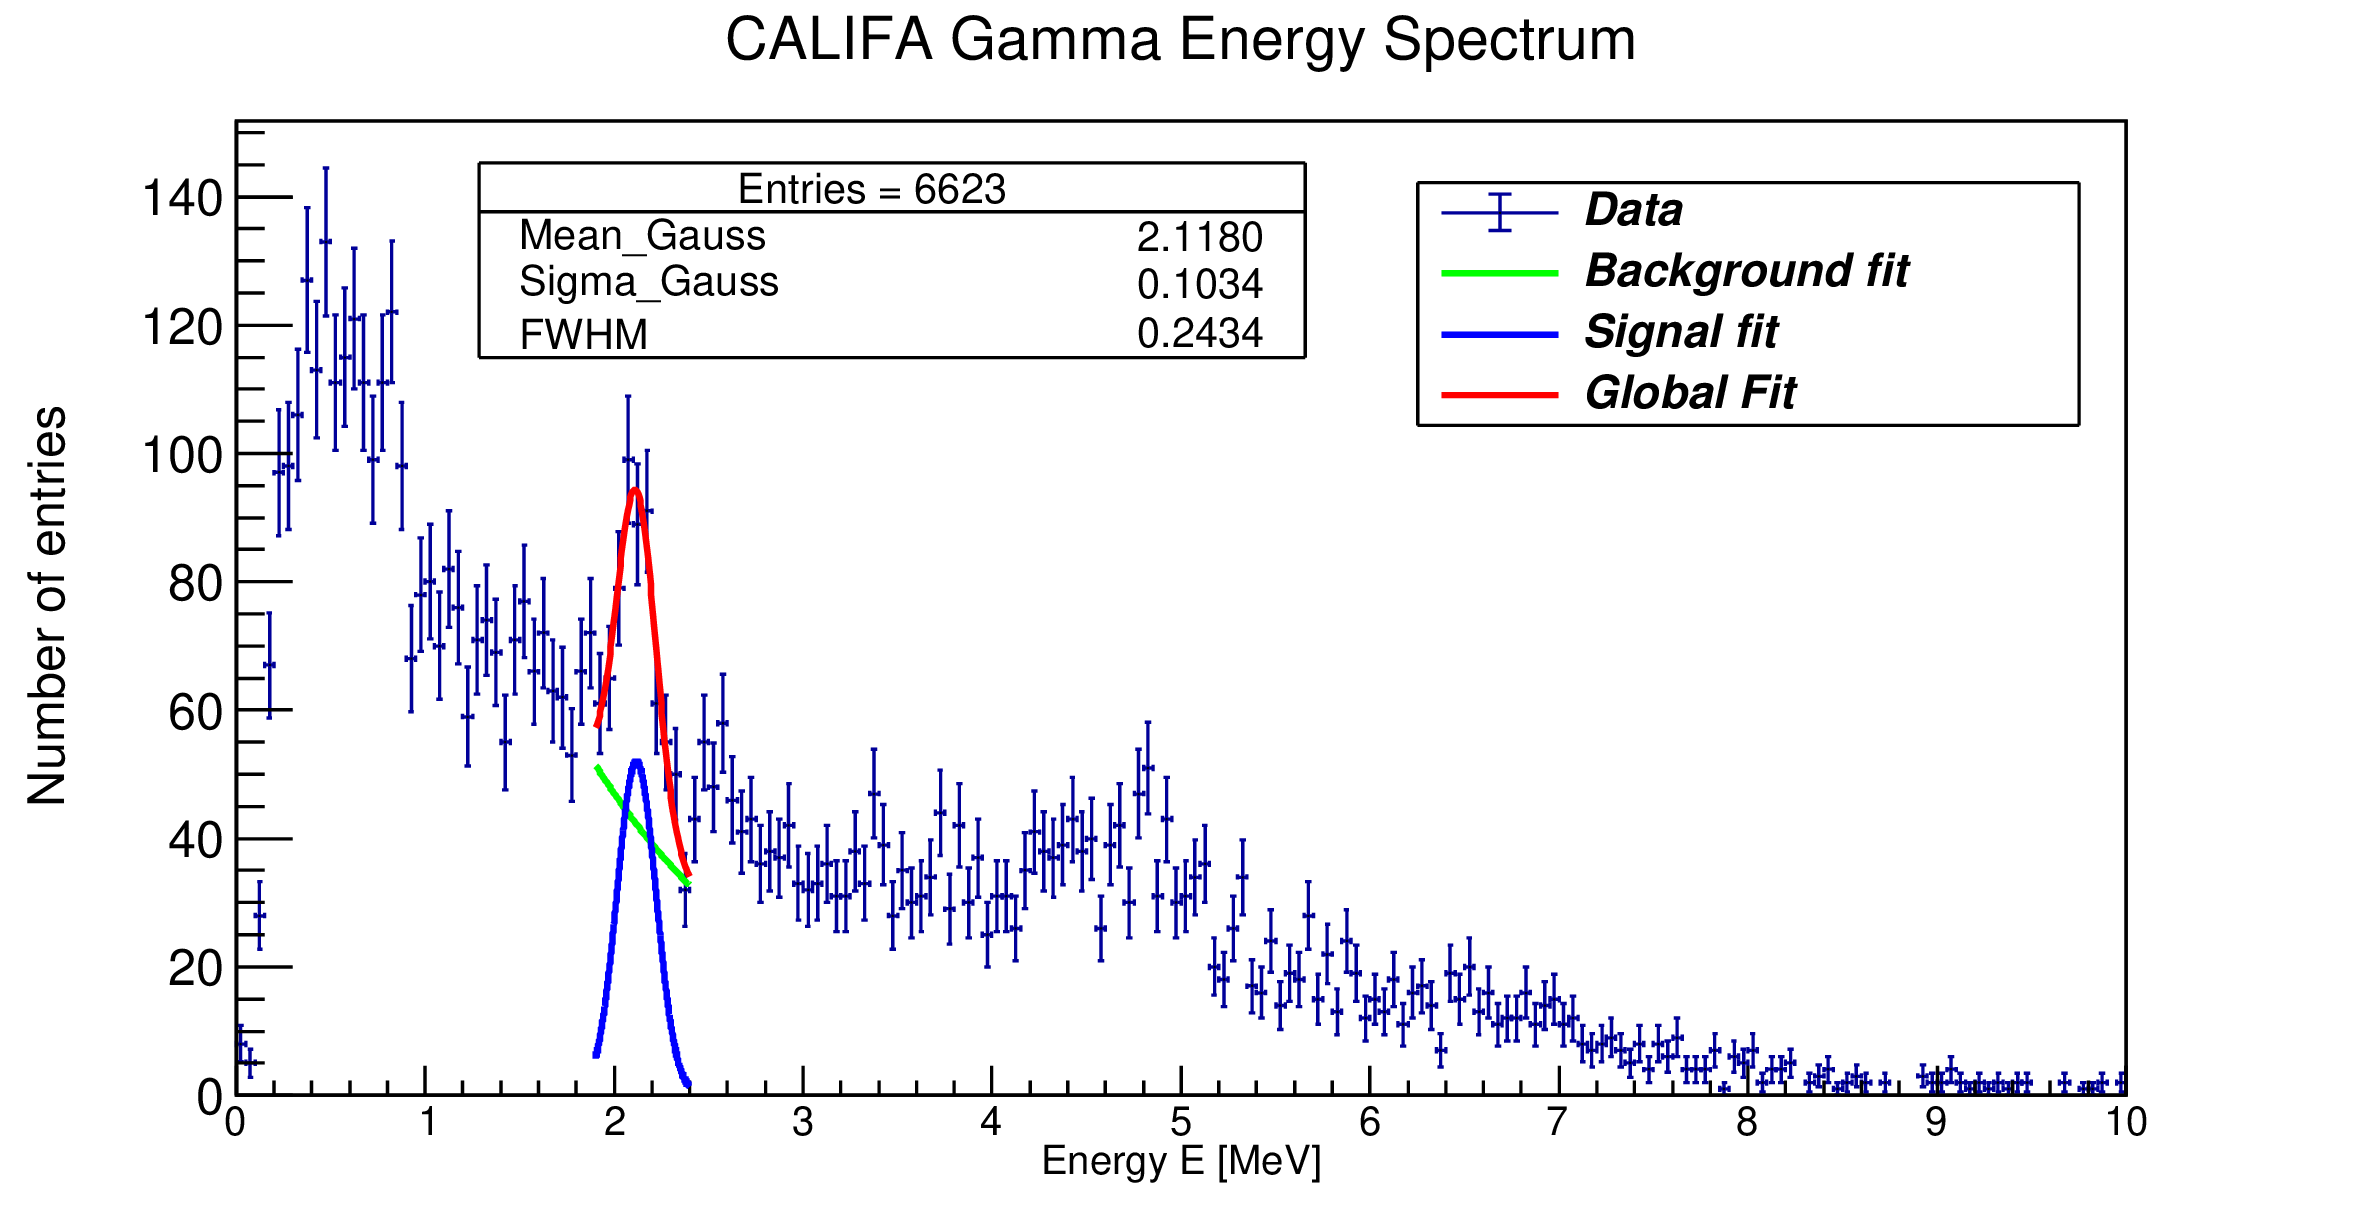
\includegraphics[width=\textwidth,keepaspectratio=true]{Figures/gamma_spec_12c_p2p_11b.png}
    \caption{
Doppler-corrected $\gamma$-ray spectrum in coincidence with the $^{12}\mathrm{C}(p,2p)^{11}\mathrm{B}$ quasi-free scattering reaction. The prominent peak at $E_{\gamma} \approx 2.1\,\mathrm{MeV}$ corresponds to the de-excitation of the $^{11}\mathrm{B}$ nucleus from its first excited state ($1/2^-$) to the ground state. This peak is fitted with a Gaussian function (blue), while the underlying background is described by an exponential distribution (green). A broader and less well-defined structure is observed at $E_{\gamma} \approx 5\,\mathrm{MeV}$, associated with the de-excitation of the $3/2^-$ state.
    }
    \label{fig:gamma_spec_12c_p2p_11b}
\end{figure}
The resulting Doppler-corrected $\gamma$-ray spectrum is presented in Figure~\ref{fig:gamma_spec_12c_p2p_11b}, which was obtained after applying the following reaction selection criteria:
\begin{itemize}
  \item Identification of the $^{11}\mathrm{B}$ fragment via time-of-flight measurements between the START detector and the TOFW (Sofia), as detailed in Section~\ref{sec:frag_ident}.
  \item Detection of two high-energy hits corresponding to protons, each with an energy deposition $E_{\text{hit}} > 30\,\mathrm{MeV}$.
\end{itemize}
In Figure~\ref{fig:gamma_spec_12c_p2p_11b}, both peaks associated with the de-excitation of the $^{11}\mathrm{B}$ nucleus from the $1/2^-$ and $3/2^-$ excited states are visible. From the fit to the $1/2^-$ peak, an energy resolution of approximately $0.24\,\mathrm{MeV}$ (FWHM) is extracted.

According to the detector specifications, the expected crystal-wise relative energy resolution is given by \(\Delta E / E = \frac{6\%}{\sqrt{E/\mathrm{MeV}}}\), which for a $2.1\,\mathrm{MeV}$ $\gamma$-ray corresponds to an ideal resolution of about $0.09\,\mathrm{MeV}$ (FWHM). The observed deviation from this expected value is non-negligible and can be attributed to several experimental and geometrical effects.

First, the Doppler correction relies on the reconstructed polar angle $\theta$ of the $\gamma$-ray, derived from the position of the crystal with the highest energy deposition within the detected cluster. However, this may not correspond to the actual primary interaction point of the photon within the scintillator. This spatial uncertainty becomes increasingly relevant for large opening angles, leading to additional broadening of the reconstructed energy peak.

Second, mechanical factors such as slight tilts or misalignments of the CALIFA detector halves, as well as minor displacements of individual crystals within the carbon alveolar frame, may further contribute to the degradation of energy resolution.

The broader and less well-defined peak at $E_{\gamma} \approx 5\,\mathrm{MeV}$, associated with the $3/2^-$ state, was not fitted due to its complex structure. This broadening is likely a result of reduced cluster reconstruction efficiency for higher-energy $\gamma$-rays. In particular, for photon energies exceeding the pair production threshold (\(E_{\gamma} > 2 m_e c^2 \approx 1.022\,\mathrm{MeV}\)), electron-positron pair production becomes a significant interaction mechanism. Above \(E_{\gamma} \gtrsim 6\,\mathrm{MeV}\), it becomes dominant. These interactions can result in spatially separated energy depositions or partial energy loss due to annihilation photons escaping detection. Consequently, this can impair both the accuracy of cluster reconstruction and the effectiveness of Doppler correction, leading to a smeared peak structure.

As anticipated, no enhancement is observed around $4.4\,\mathrm{MeV}$, which would correspond to the population of the $5/2^-$ state. This is consistent with the quasi-free scattering mechanism, which does not favor the population of such states involving complex multi-nucleon configurations.

It should be emphasized that this experiment represents the first measurement campaign using CALIFA in its final mechanical configuration. The successful reconstruction of Doppler-corrected $\gamma$-ray spectra in coincidence with the $^{12}\mathrm{C}(p,2p)^{11}\mathrm{B}$ reaction serves as a proof of concept, demonstrating the capability of CALIFA as a key instrument for performing correlated measurements of $\gamma$-rays and light charged particles. These results contribute significantly to the overarching goal of achieving full kinematic reconstruction of nuclear reactions under investigation.


\subsection{Fission via Quasi-Free Scattering reaction}\label{sec:fission_qfs}
In 2021, the S455 experiment conducted at the R$^3$B experiment marked a significant advancement in experimental nuclear physics through the realization of an unprecedented fission study employing quasi-free scattering as a reaction mechanism. This approach induces fission via particle-hole excitations, which can span excitation energies from a few MeV up to several tens of MeV.\newline
Since the discovery of the nuclear fission by O. Hahn and F. Straßmann 1939~\cite{hahn1939nachweis} and the first interpretations of the underlying process by Lise Meitner and R. O. Frisch~\cite{meitner1939disintegration} and the theoretical approach of Bohr and Wheeler~\cite{bohr1939phys} with help of the liquid drop model numerous fission experiments were carried out for better understanding of fission as consequence of a dynamic instability of the considered nucleus.\newline
To induce fission an activation energy $T_a$ has to be supplied to overcome the Coulomb wall. The final energy released inform of kinetetic energy of the fission products $T_f$ is given by:
\[
Q = (m_i -m_f)c^2 = T_f - T_a
\]
where $m_i$ is the initial mass of the fissile nucleus and $m_f$ the sum of the masses of the fission products. Figure X shows the potential curve for the fission process into two fission fragments.\newline
In case of low fission barriers $T_a$ \textit{spontaneous fission}(s.f.) may occur. For many other nuclei a higher potential wall is expected  where no spontaneous fission is observed. In that case a relatively small energy $T_a$ needs to be supplied to \textit{induce fission}.
From previous fission experiments fission yields for a large range of exotic nuclei were measured together with the mass/charge distribution of the (two) fission fragments. It has been observed that there are distinct regions of symmetric mass distribution and as well as asymmetric regions which cannot be understood by liquid drop model approximations. Moreover many different processes associated with fission have shown that the fission barrier does not always have a single maximum as predicted by the liquid drop model~\cite{bassani2005encyclopedia}. It follows that, within the framework of theoretical models, the description must generally combine concepts from both the liquid-drop model and the shell model giving high importance to the fine structure of the topography of the potential-energy surface (PES) as shownn in Figure~\ref{fig:drop_shell_model}, implemented in scission models which focuses on the specific configuration of the fissioning nucleus just before it splits into fragments, considering factors like potential energy and shell effects~\cite{pacsca2016possible,andreev2012mass,moller2012calculated}.\newline

\begin{figure}[htpb]
    \centering
    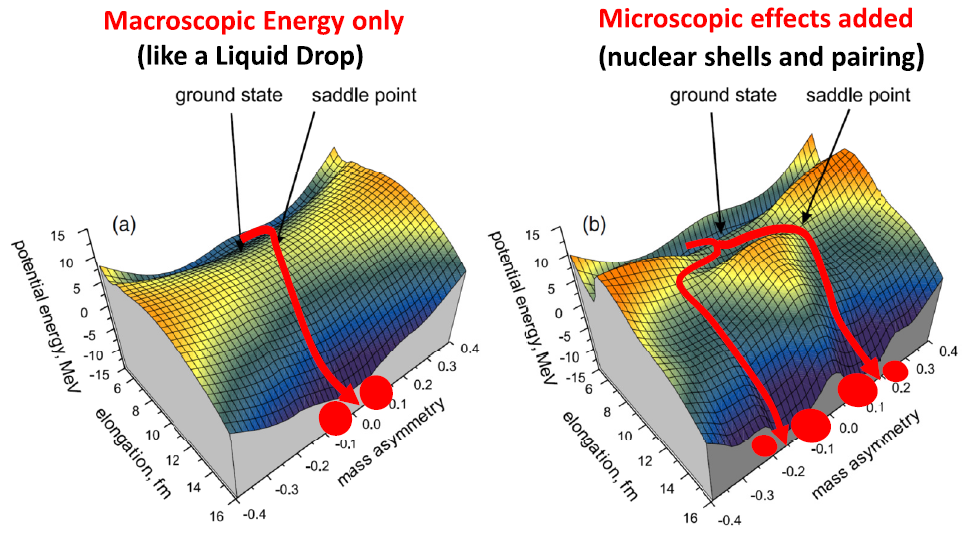
\includegraphics[width=\textwidth,keepaspectratio=true]{Figures/liquid_drop.png}
    \caption{
    Most probable fission paths (red arrows) in the a) liquid drop model which postulates symmetric fission fragment masses. b) includes shell effects introducing asymmetry in the fragment's mass distribution. Figure from~\cite{popescu2021review}. 
    }
    \label{fig:drop_shell_model}
\end{figure}

However, when microscopic effects—such as nuclear shell corrections and pairing interactions—are taken into account, the PES becomes substantially more complex and requires higher-resolution experimental techniques for validation.\newline
To test these more nuanced theoretical predictions, a detailed and differential mapping of the PES is necessary. Fission induced via QFS reactions offers a promising experimental approach for this purpose. In QFS-induced fission, the projectile interacts with an individual nucleon within the target nucleus, leading to localized and controlled excitation of the residual system. This allows for event-by-event measurement of the fission process, enabling a direct correlation between the excitation energy and the resulting fission fragment charge and mass distributions, as well as the fission probabilities.\newline
Such differential data facilitate a more precise determination of the temperature dependence of the fission process and the underlying fission barrier heights for exotic, neutron-rich heavy nuclei. By systematically analyzing these correlations, QFS-induced fission can provide critical constraints on theoretical models of the PES and improve our understanding of fission dynamics far from stability.\newline
In the S455 experiment, as proof of principle, for fission via quasi-free scattering the reaction $^{238}U(p,2pf)$ was analyzed, with an intermediate excited nucleus Protactinum (Pa*) which undergoes fission. An overview of the reaction mechanism is shown in Figure~\ref{fig:drop_shell_model}.\newline 
\begin{figure}[htpb]
    \centering
    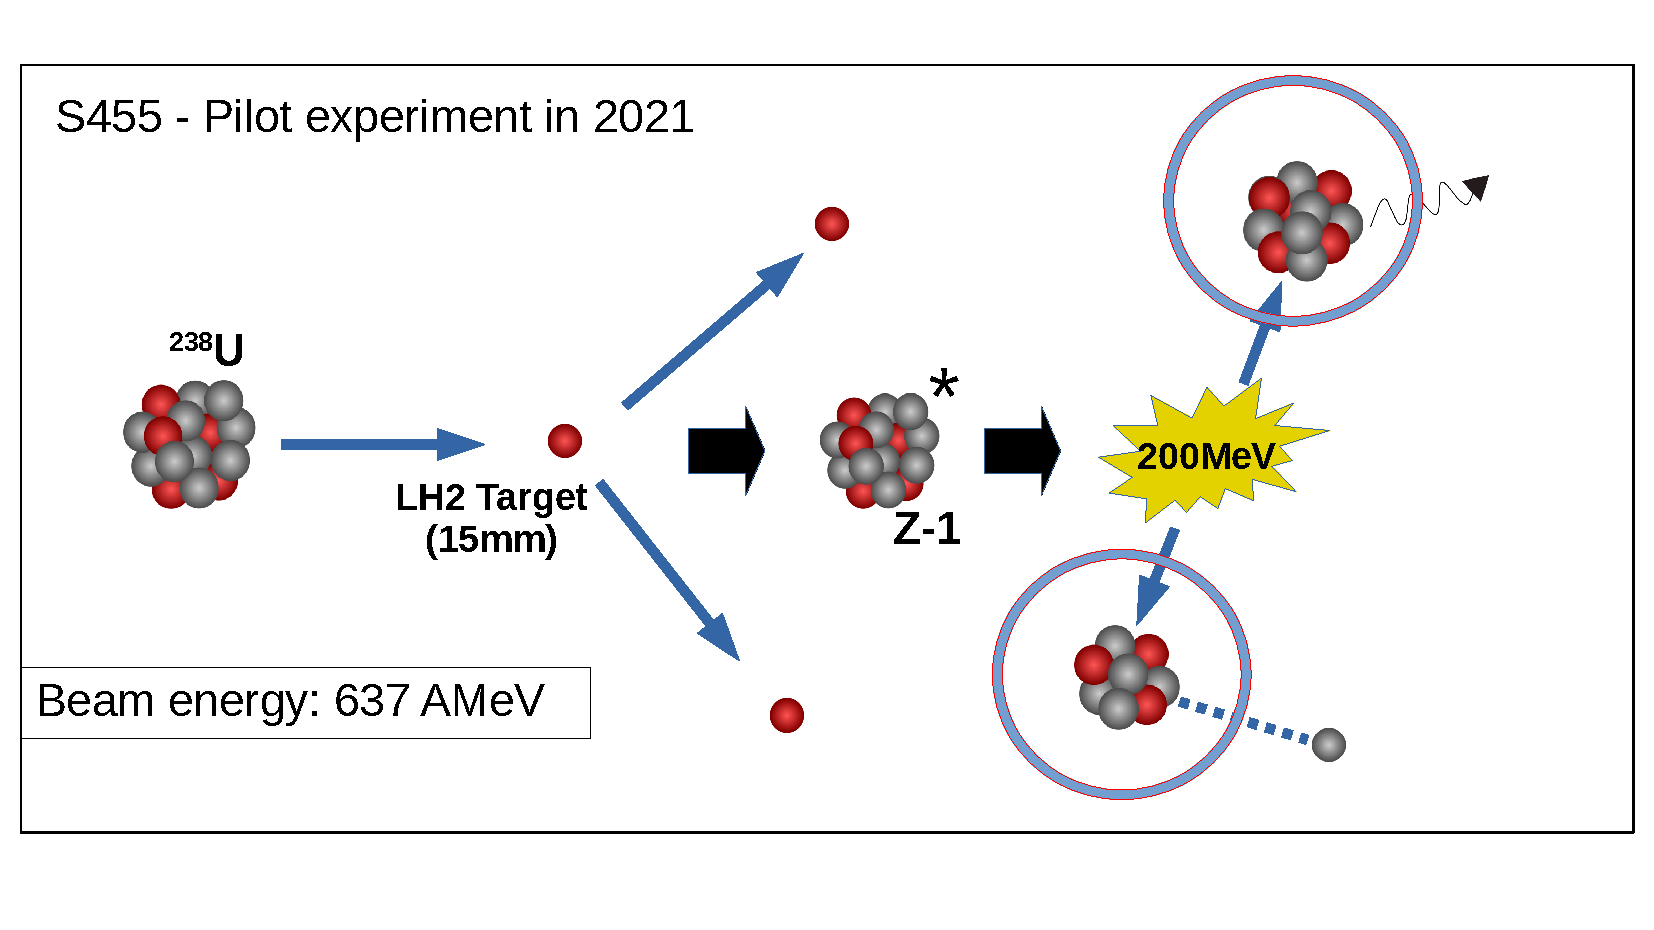
\includegraphics[width=\textwidth,keepaspectratio=true]{Figures/overview_exp_2021_s455.pdf}
    \caption{
    Overview of reaction mechanism $^{238}U$(p,2pf) in inverse kinematics.
    }
    \label{fig:drop_shell_model}
\end{figure}
The realization of the proposed experiment required a finely tuned  setup was needed for a complete identification of the fission fragments and the determination of the neutrons emitted in coincidence. Moreover a  precise measurement of the momentum of the knockout protons was required for a full charcterization of the fissioning process.\newline
Central detector for the simultaneous charge measurement of the fission fragments is the TWIN MUSIC thanks to its four-section geometry (for more details see: Section~\ref{sec:ionisation_chambers}). %TODO find charge resolution of TWIN
However the energy/charge calibration employs many fine-tuning steps to retrieve the final charges of the fission products:
\begin{itemize}
\item Anode- and section wise calibration
%TODO: more; maybe also some plots you have

\end{itemize}
The final calibration of the TWIN MUSIC was carried out by our colleagues from University Spain,Valencia,Santiago.\newline
The key detector for the identification of the quasi-free scattering part of the reaction was the CALIFA calorimeter. For this experiment the CALIFA DAQ was operated for the first time in multi-event readout mode since high CALIFA event rates were expected and from the experience from the S444 experiment, where CALIFA was operated in a fully self triggered mode, which slowed down the event-building rate and capabilities of the full R3B DAQ\footnote{For more details about the CALIFA DAQ readout modes see~\cite{pklenze}, Section 5.2}.\newline
However, for offline analyis this configuration posed several data unwrapping steps to correctly assign the hits within the asynchronous multi-event readout blocks to the according recorded events. 



%
%Over the past decades, Coulomb-induced fission reactions in inverse kinematics have served as a powerful tool to investigate fission dynamics and the nuclear structure of both stable and unstable heavy nuclei at large deformations. These reactions, however, provide only averaged information over many fission events, thereby limiting their ability to resolve the detailed topography of the potential-energy surface (PES). Consequently, they offer only indirect access to the fission barrier through measurements of integrated fission yields, making it difficult to probe finer aspects of fission dynamics.\newline
%
%
%Coulomb-induced fission has confirmed the broad features predicted by macroscopic models such as the liquid-drop model, which typically exhibits a single, smooth rise in the PES leading to fission, as illustrated in Figure 1.
%
%-> shortly explain the challenges behind, idea should be in the theory part. Also mention that this was complementary experiment to Coulex Exp, where nature paper was submitted
%-> mention that TUM Munich group was strongly involved
%-> Charge reconstruction is done, mention the papers and publications
%-> One really interesting aspect would have been to pick out specific reaction channels, eg. with one fission fragment being a thin isotope and look at the gamma spectrum. 
%-> the issue there is of course that precise thin isotope cannot be selected yet. But from CALIFA side this was motivation to improve the clustering algorithm, especially for fission reactions, where you have lot more hits in CALIFA. And there especially looking at low energy hits from gammas, which can be quite sparse.
%-> This should then be the introduction for the next section about clustering.
\newpage
